\documentclass[a4paper,12pt]{article}
% -------------------------------------------------------------------
%                  Essential packages (used in template)
% -------------------------------------------------------------------

\usepackage[utf8]{inputenc}                   % Allow Umlauts (ä, ö, ü)
\usepackage[ngerman]{babel, translator}       % German LaTeX-intern descriptors (Abbildungen, ...)
\usepackage{mathptmx}                         % Font "Times New Roman" in mathematical Environments
\usepackage{courier}                          % Support the use of font "Courier" (used in listings)
\usepackage[T1]{fontenc}                      % Change LaTeX font encoding to support modern fonts
\usepackage{fix-cm}                           % Fix sizes at which CM and EC fonts can be used

\usepackage{geometry}                         % Change text bounds on a per-page basis
\usepackage{fancyhdr}                         % Allow easy customization of headers and footers

\usepackage[ddmmyyyy]{datetime}               % Reformat times from LaTeX commands like \today

\usepackage[usenames,dvipsnames]{xcolor}      % Support text colorization

\usepackage{colortbl}                         % Support applying colors to tables
\usepackage{array}                            % Tables with fixed column size
\usepackage{longtable}                        % Support multi-page tables
\usepackage{multicol}                         % Additional settings for \multicolumn
\usepackage{multirow}                         % Additional settings for \multirow

\usepackage[hyphens,obeyspaces,spaces]{url}   % Allow urls to have line breaks at "-"
\usepackage{hyperref}                         % Clickable hyperlinks in Table of Contents
\usepackage{microtype}                        % Enable "Blocksatz"

\usepackage{float}                            % Support for table H option
\usepackage{floatflt}                         % Support text wrapping around floating environments
\usepackage{wrapfig}                          % Support text wrapping around figures

\usepackage{graphicx}                         % Support including graphics environments for images
\usepackage{caption}                          % Provide greater customization around captions
\usepackage{subcaption}                       % Caption support for subfigures

\usepackage[onehalfspacing]{setspace}         % Set line spacing to be 1.5x the default
\usepackage{listings}                         % Code block support for LaTeX

\usepackage[titles]{tocloft}                  % More options to modify list of figures & tables
\usepackage{nomencl}                          % Support for nomenclatures ("Symbolverzeichnis")

\usepackage{amsmath}                          % Includes a plethora of mathematical packages 
\usepackage{amssymb}                          % Source mathematical symbols like \sin
\usepackage{amsthm}                           % Better theorems
\usepackage{upgreek}                          % Use \Upomega to get a straight \Omega
\usepackage{siunitx}                          % Unified support for si units

\usepackage{ifthen}                           % Support better if statements in LaTeX
\usepackage{etoolbox}                         % Easily patch commands

% Support list of acronyms and glossary
\usepackage[
  toc,
  nogroupskip,
  nonumberlist,
  nopostdot,
  acronyms,
  shortcuts,
  translate=babel
]{glossaries}

% Track the total count of different environments
% Needs to be imported because LaTeX resets these counter on a chapter basis
\usepackage[figure,table,lstlisting,xspace]{totalcount}

% Annotate different information directly into the document
\setlength{\marginparwidth}{2cm}
\usepackage[
  colorinlistoftodos,
  prependcaption,
  textsize=tiny
]{todonotes}

% -------------------------------------------------------------------
%                 Useful packages (not used in template)
% -------------------------------------------------------------------

\usepackage{pdfpages}                         % Include existing PDFs into the work

% Create electrical diagrams within LaTeX
\usepackage[
  european,
  oldvoltagedirection,
  straightvoltages,
  siunitx
]{circuitikz}
% Disable single lines at the start of a paragraph (Schusterjungen)
\clubpenalty=10000

% Disable single lines at the end of a paragraph (Hurenkinder)
\widowpenalty=10000
\displaywidowpenalty=10000

% Fixed size table columns
\newcolumntype{L}[1]{>{\raggedright\arraybackslash}p{#1}}
\newcolumntype{C}[1]{>{\centering\arraybackslash}p{#1}}
\newcolumntype{R}[1]{>{\raggedleft\arraybackslash}p{#1}}

\renewcommand{\arraystretch}{1.2}                       % Distance between lines in tables

\captionsetup{justification=raggedright}                % Align captions to the left

\setcounter{secnumdepth}{3}                             % Only allow nesting 3 layers (down to subsubsections)

% Unit-related setup for siunitx
\sisetup{
  locale=DE,                   % Use German notation (comma instead of point delimiter for floats)
  per-mode=fraction,           % Switch display to use \frac instead of x^{-1}
  fraction-function=\tfrac,    % Use amsmath's tfrac macro for unit fractions
}

% -------------------------------------------------------------------
%                     Usability & visual changes
% -------------------------------------------------------------------

% Page margins
\geometry{
  left=2.5cm,
  right=2.5cm,
  top=2.5cm,
  bottom=3cm
}

% Create a better looking header and footer
\pagestyle{fancy}
\fancyhf{}
\lhead{\nouppercase{\leftmark}}
\rfoot{\thepage}

% Automatically generate a box around figure environments
%\floatstyle{boxed}
%\restylefloat{figure}

% Set toc sections to be clickable
\hypersetup{
  colorlinks,
  citecolor=black,
  filecolor=black,
  linkcolor=black
}

\frenchspacing                                          % Insert one space after a sentence, not 2

\renewcommand{\UrlFont}{\color{blue}\rmfamily\itshape}  % URLs should be displayed in blue
\renewcommand{\dateseparator}{.}                        % Dates are written like 01.01.1970, not 01-01-1970

\addto{\captionsngerman}{
  \renewcommand*{\figurename}{Abb.}                     % Figures should be displayed as "Abb. x"
  \renewcommand*{\tablename}{Tab.}                      % Tables  should be displayed as "Tab. x"
  \renewcommand*{\lstlistingname}{Code}                 % Code    should be displayed as "Code x"
  \renewcommand*{\nomname}{Symbolverzeichnis}           % Nomenclature in German is "Symbolverzeichnis"
}

% -------------------------------------------------------------------
%                        Code listing setup
% -------------------------------------------------------------------

\lstset{
  basicstyle=\small\ttfamily\color{black},              % Font size used for the code
  commentstyle=\ttfamily\color{gray},                   % Comment style
  keywordstyle=\ttfamily\color{blue},                   % Keyword style
  stringstyle=\color{ForestGreen!30!LimeGreen},         % String literal style
  frame=single,                                         % Add a frame around the code
  showstringspaces=false,                               % Don't underline spaces within strings only
  captionpos=b,                                         % Set caption-position to bottom
  backgroundcolor=\color{white},                        % Background color
}

% To style lstlistlisting like the lof, you first have to register it
% to tocloft, as mentioned in https://tex.stackexchange.com/a/27648/27635
\makeatletter
\begingroup\let\newcounter\@gobble\let\setcounter\@gobbletwo
  \globaldefs\@ne \let\c@loldepth\@ne
  \newlistof{listings}{lol}{\lstlistlistingname}
\endgroup
\let\l@lstlisting\l@listings
\makeatother

% -------------------------------------------------------------------
%                         Redefining geometry
% -------------------------------------------------------------------

% Figures
\renewcommand{\cftfigpresnum}{\figurename~}
\renewcommand{\cftfigaftersnum}{:}
\setlength{\cftfignumwidth}{2cm}
\setlength{\cftfigindent}{0cm}

% Tables
\renewcommand{\cfttabpresnum}{\tablename~}
\renewcommand{\cfttabaftersnum}{:}
\setlength{\cfttabnumwidth}{2cm}
\setlength{\cfttabindent}{0cm}

% Listings
\renewcommand*{\cftlistingspresnum}{\lstlistingname~}
\renewcommand*{\cftlistingsaftersnum}{:}
\settowidth{\cftlistingsnumwidth}{\cftlistingspresnum}
\addtolength{\cftlistingsnumwidth}{1cm}
\setlength{\cftlistingsindent}{0cm}

\setlength{\parindent}{0cm}                             % Don't indent start of paragraph
\setlength{\parskip}{6pt}                               % Lines are seperated by 6pt

\setlength{\headheight}{1.25cm}
\setlength{\footskip}{1cm}
\setlength{\headsep}{1cm}

% -------------------------------------------------------------------
%                    Custom counters & commands
% -------------------------------------------------------------------

\newcounter{countacronym}
\DeclareTotalCounter{countacronym}
\newcommand*{\acr}[1]{\acrshort{#1}\stepcounter{countacronym}}
\newcommand*{\Acr}[1]{\acrlong{#1}\stepcounter{countacronym}}

\newcounter{countnomen}
\DeclareTotalCounter{countnomen}
\newcommand*{\nomen}[2]{\nomenclature{#1}{#2}\stepcounter{countnomen}}
\newcommand{\nomunit}[1]{\renewcommand{\nomentryend}{\hspace*{\fill}#1}}
\newcommand{\nomsi}[1]{\nomunit{[\si{#1}]}}

% Count number of references to the glossary
\newcounter{countglossary}
\DeclareTotalCounter{countglossary}
\pretocmd{\Gls}{\stepcounter{countglossary}}{}{}
\pretocmd{\gls}{\stepcounter{countglossary}}{}{}
\pretocmd{\Glspl}{\stepcounter{countglossary}}{}{}
\pretocmd{\glspl}{\stepcounter{countglossary}}{}{}

% TODO annotations
\newcounter{counttodo}
\DeclareTotalCounter{counttodo}
\newcommand{\note}[2][]{
  \todo[color=green!25,bordercolor=green,tickmarkheight=3pt,#1]{#2}
  \stepcounter{counttodo}
}
\newcommand{\unsure}[2][]{
  \todo[color=Plum!25,bordercolor=Plum,tickmarkheight=3pt,#1]{#2}
  \stepcounter{counttodo}
}
\newcommand{\change}[2][]{
  \todo[color=blue!25,bordercolor=blue,tickmarkheight=3pt,#1]{#2}
  \stepcounter{counttodo}
}

\newcommand{\imgref}[1]{\hyperref[#1]{Abbildung~\getrefnumber{#1}}}
\newcommand{\tabref}[1]{\hyperref[#1]{Tabelle~\getrefnumber{#1}}}
\newcommand{\coderef}[1]{\hyperref[#1]{Code~\getrefnumber{#1}}}
\newcommand{\mathref}[1]{\hyperref[#1]{Gleichung~\getrefnumber{#1}}}
\newcommand{\secref}[1]{\hyperref[#1]{Abschnitt~\getrefnumber{#1}}}


% Preload custom user settings & packages
\IfFileExists{./Custom.tex}{\include{Custom}}{}

\newcommand{\startHSCdocument}[1][]{

  % Register different entries: glossary, nomenclature, acronyms
  \makeglossaries
  \hyphenation{}

  \newacronym{cpu}{CPU}{Central Processing Unit}
\newacronym{cuda}{CUDA}{Compute Unified Device Architecture}
\newacronym{gpu}{GPU}{Graphics Processing Unit}
\newacronym{ki}{KI}{Künstliche Intelligenz}
\newacronym{ppo}{PPO}{Proximal Policy Optimization}
\newacronym{relu}{ReLU}{Rectified Linear Unit}
\newacronym{gpt}{GPT}{Generative Pre-trained Transformer}
\newacronym{rl}{RL}{Reinforcement Learning}
\newacronym{api}{API}{Application Programming Interface}
  \makenomenclature
  \nomenclature[01]{\textbf{Symbol}}{\textbf{Bedeutung} \nomunit{\textbf{[phys. Einheit]}}}

  \newglossaryentry{Kästchen}
{
	name=Kästchen,
	plural=Kästchen,
	description={Ein Kästchen beschreibt ein Rechteck des Spielbretts von \textit{"Ganz schön clever"}, welches ausgefüllt werden kann, wenn bestimmte Bedingungen erfüllt sind.}
}
\newglossaryentry{Feld}
{
	name=Feld,
	plural=Felder,
	description={Ein Feld ist eines der farbigen Felder (gelb, blau, grün, orange, lila) auf dem Spielbrett von \textit{"Ganz schön clever"}.}
}
\newglossaryentry{Extra-Wahl}
{
	name=Extra-Wahl,
	plural=Extra-Wahlen,
	description={Eine Extra-Wahl beschreibt eine Wahl mithilfe des Extra-Wahl-Bonus oder vom Silbertablett eines Mitspielers.}
}
\newglossaryentry{Wahl}
{
	name=Wahl,
	plural=Wahlen,
	description={Eine Wahl beschreibt den Vorgang bei dem ein Würfel oder eine Boni gewählt wird, um eines der Kästchen auf dem Spielbrett auszufüllen.\newpage}
}
\newglossaryentry{Bonusrunde}
{
	name=Bonusrunde,
	plural=Bonusrunden,
	description={Eine Bonusrunde ist eine Runde bei der der Rundenablauf nicht wie üblich inkrementiert wird. Diese Einteilung ist notwendig, da bei Wahlen mit Boni oder vom Silbertablett eines Mitspielers andere Regeln gelten, als bei Wahlen nach dem eigenen Würfen. Alle Wahlen, bis auf Wahlen nach einem gewöhnlichen eigenen Wurf, sind Wahlen in einer Bonusrunde.}
}
\newglossaryentry{ungültige Aktion}
{
	name=ungültige Aktion,
	plural=ungültige Aktionen,
	description={Eine ungültige Aktion ist eine Aktion, die im normalen Spielablauf nicht stattfinden würde. Ungültige Aktionen treten auf, wenn dem Modell keine gültige Aktion zur Auswahl steht.}
}
\newglossaryentry{ungültiger Würfel}
{
	name=ungültiger Würfel,
	plural=ungültige Würfel,
	description={Ein ungültiger Würfel ist ein Würfel, der nicht mehr zur Wahl steht und nicht mehr geworfen wird.}
}
\newglossaryentry{Modell}
{
	name=Modell,
	plural=Modelle,
	description={Ein Modell beschreibt den Teil einer Künstlichen Intelligenz, der im Stande ist, Vorhersagen zu treffen}
}
\newglossaryentry{Agent}
{
	name=Agent,
	plural=Agenten,
	description={Ein Agent ist die ausführende Instanz der Künstlichen Intelligenz. Er nimmt die Umgebung wahr und führt Aktionen in dieser aus.}
}

  % Register actual document
  \begin{document}
  \shorthandoff{"}

  % ===========================================================================
  %                             Document header
  % ===========================================================================

  \newgeometry{
    left=2.5cm,
    right=2.5cm,
    top=2.5cm,
    bottom=2.5cm
  }

  % Correctly determine type of document and format in respective header
  \newcommand{\DocumentType}{#1}

  \begin{titlepage}
    \ifthenelse{\equal{#1}{Praxisbericht}}
      {\centering

\includegraphics[width=.8\textwidth]{framework/Logo_HS_Coburg}

\begin{Large}
  Hochschule für angewandte Wissenschaften Coburg\\
  Fakultät Elektrotechnik und Informatik\par
\end{Large}
\vspace{1.5cm}

\Large{Studiengang: \Studiengang}
\vspace{1.5cm}

\Large{Praxisbericht}
\vspace{1cm}

\huge{\Autorenname}
\vspace{1.5cm}

\begin{table}[H]
  \begin{tabular}{|L{3cm}|L{11cm}|}
  \hline
  Unternehmen & \Unternehmen        \\
              & \Abteilung          \\
              & \Strasse            \\
              & \Ort                \\
  \hline
  Zeitraum    & \Beginn \ bis \Ende \\
  \hline
  \end{tabular}
\end{table}

\large{Abgabe des Berichts: \Abgabe}

\begin{table}[H]
  \begin{tabular}{|L{3cm}|L{6cm}|L{5cm}|}
    \multicolumn{3}{l}{Freigabe zur Vorlage des Praxisberichts an der HS Coburg:} \\
    \hline
    Betreuer & \Betreuer & \\
    \hline
    Funktion & \Funktion & \textbf{\textit{Ort, Datum}}\\
    \hline
    Telefon & \Telefon & \\
    \cline{1-2}
    Email & \Email & \\
    \hline
    & & \textbf{\textit{Unterschrift Betreuer}}\\
    \hline
  \end{tabular}
\end{table}
}
      {
        \ifthenelse{\equal{#1}{Bachelorarbeit}}
          {\centering

\includegraphics[width=.8\textwidth]{framework/Logo_HS_Coburg}

\begin{Large}
  Hochschule für angewandte Wissenschaften Coburg\\
  Fakultät Elektrotechnik und Informatik\par
\end{Large}
\vspace{1.5cm}

\Large{Studiengang: \Studiengang}
\vspace{1.5cm}

\Large{\DocumentType}
\vspace{1cm}

\Huge{\Titel}
\vspace{2cm}

\huge{\Autorenname}
\vspace{2cm}

\Large{Abgabe der Arbeit: \Abgabe}

\Large{Betreut durch:}

\Large{\Betreuer, Hochschule Coburg}

\newpage
\begin{abstract}
\raggedright
Ziel dieser Arbeit war es, eine Künstliche Intelligenz, für das Brettspiel \textit{"Ganz schön clever"}, zu entwickeln und den Entwicklungs- sowie Trainingsprozess zu evaluieren.
Diese Künstliche Intelligenz wurde erfolgreich entwickelt und kann das Brettspiel \textit{"Ganz schön clever"} gut spielen. Zunächst wurde dafür ein Prototyp entwickelt, welcher dann schrittweise erweitert wurde, um die gesamte Komplexität des Spiels zu erfassen.

Das Brettspiel \textit{"Ganz schön clever"} ist ein Würfelspiel, welches eine hohe Komplexität aufweist. Diese kommt vor allem durch die vielen Aktionsmöglichkeiten des Spielers und die multiplen Zusammenhängen innerhalb des Belohnungssystems zustande. Außerdem weist es eine hohe Stochastizität auf, welche die Komplexität weiter erhöht.

Für die Implementierung der Künstlichen Intelligenz wurde Deep Reinforcement Learning verwendet. Während der Implementierungsphase kam es zunächst zu einem Problem, bei dem die Künstliche Intelligenz es nur schwer selbstständig schaffte, gültige Aktionen zu wählen, welche nicht zum Abbruch des Spiels geführt haben. Dieses Vorgehen, bei dem das Spiel nach Wahl einer ungültigen Aktion abgebrochen wurde, wurde nach einigen Tagen verworfen. Daraufhin wurde zunächst ein Verfahren implementiert, bei dem das Spiel bei ungültigen Aktionen nicht sofort abgebrochen, sondern negativ belohnt wurde. Diese Vorgehen stellte sich als gut geeignet heraus, wurde aber schnell von einem Vorgehen, welches eine Aktionsmaske verwendet abgelöst. Im Folgenden wurde eine Aktionsmaske implementiert, welche gewährleistet, dass nur gültige Aktionen gewählt werden können. Die Performanz stieg mit diesem Vorgehen von vorher durchschnittlich ungefähr 60 Prozent der Maximalpunktzahl auf 75 Prozent. Zudem ergaben sich Schwierigkeiten bei der Erweiterung des Runden-Systems und viele weitere Probleme, die behoben werden mussten.

Das Ergebnis des finalen Trainings war eine Künstliche Intelligenz, welche durchschnittlich 208 Punkte mit einer Standardabweichung von 31 im Spiel erzielt. Im Vergleich dazu erzielten menschliche Spieler in einem Test im Durchschnitt lediglich 160 Punkte.
\end{abstract}
\newpage}
          {
            \ifthenelse{\equal{#1}{Masterarbeit}}
              {\centering

\includegraphics[width=.8\textwidth]{framework/Logo_HS_Coburg}

\begin{Large}
  Hochschule für angewandte Wissenschaften Coburg\\
  Fakultät Elektrotechnik und Informatik\par
\end{Large}
\vspace{1.5cm}

\Large{Studiengang: \Studiengang}
\vspace{1.5cm}

\Large{\DocumentType}
\vspace{1cm}

\Huge{\Titel}
\vspace{2cm}

\huge{\Autorenname}
\vspace{2cm}

\Large{Abgabe der Arbeit: \Abgabe}

\Large{Betreut durch:}

\Large{\Betreuer, Hochschule Coburg}

\newpage
\begin{abstract}
\raggedright
Ziel dieser Arbeit war es, eine Künstliche Intelligenz, für das Brettspiel \textit{"Ganz schön clever"}, zu entwickeln und den Entwicklungs- sowie Trainingsprozess zu evaluieren.
Diese Künstliche Intelligenz wurde erfolgreich entwickelt und kann das Brettspiel \textit{"Ganz schön clever"} gut spielen. Zunächst wurde dafür ein Prototyp entwickelt, welcher dann schrittweise erweitert wurde, um die gesamte Komplexität des Spiels zu erfassen.

Das Brettspiel \textit{"Ganz schön clever"} ist ein Würfelspiel, welches eine hohe Komplexität aufweist. Diese kommt vor allem durch die vielen Aktionsmöglichkeiten des Spielers und die multiplen Zusammenhängen innerhalb des Belohnungssystems zustande. Außerdem weist es eine hohe Stochastizität auf, welche die Komplexität weiter erhöht.

Für die Implementierung der Künstlichen Intelligenz wurde Deep Reinforcement Learning verwendet. Während der Implementierungsphase kam es zunächst zu einem Problem, bei dem die Künstliche Intelligenz es nur schwer selbstständig schaffte, gültige Aktionen zu wählen, welche nicht zum Abbruch des Spiels geführt haben. Dieses Vorgehen, bei dem das Spiel nach Wahl einer ungültigen Aktion abgebrochen wurde, wurde nach einigen Tagen verworfen. Daraufhin wurde zunächst ein Verfahren implementiert, bei dem das Spiel bei ungültigen Aktionen nicht sofort abgebrochen, sondern negativ belohnt wurde. Diese Vorgehen stellte sich als gut geeignet heraus, wurde aber schnell von einem Vorgehen, welches eine Aktionsmaske verwendet abgelöst. Im Folgenden wurde eine Aktionsmaske implementiert, welche gewährleistet, dass nur gültige Aktionen gewählt werden können. Die Performanz stieg mit diesem Vorgehen von vorher durchschnittlich ungefähr 60 Prozent der Maximalpunktzahl auf 75 Prozent. Zudem ergaben sich Schwierigkeiten bei der Erweiterung des Runden-Systems und viele weitere Probleme, die behoben werden mussten.

Das Ergebnis des finalen Trainings war eine Künstliche Intelligenz, welche durchschnittlich 208 Punkte mit einer Standardabweichung von 31 im Spiel erzielt. Im Vergleich dazu erzielten menschliche Spieler in einem Test im Durchschnitt lediglich 160 Punkte.
\end{abstract}
\newpage}
              {
                \IfFileExists{./CustomHeader.tex}{
                  \include{CustomHeader}
                }{
                  ERROR: Please use one of the following values as parameter
                  to the HSCdocument environment:\\
                  "Praxisbericht", "Bachelorarbeit", "Masterarbeit"\\

                  To create your own document header, just create a file
                  "CustomHeader.tex" in the document root.
                }
              }
          }
      }
  \end{titlepage}

  \restoregeometry

  % ===========================================================================
  %                              Page Ordering
  % ===========================================================================

  % Set image path to "Bilder" subdirectory
  \graphicspath{{Bilder/}}

  \newpage
  \setcounter{page}{2}
  \tableofcontents

  \iftotalfigures
    \newpage
    \phantomsection
    \addcontentsline{toc}{section}{\listfigurename}
    \listoffigures
  \fi

  \iftotaltables
    \newpage
    \phantomsection
    \addcontentsline{toc}{section}{\listtablename}
    \listoftables
  \fi

  \iftotallstlistings
    \newpage
    \renewcommand{\lstlistlistingname}{Codebeispielverzeichnis}
    \phantomsection
    \addcontentsline{toc}{section}{\lstlistlistingname}
    \lstlistoflistings
  \fi

  % Nomenclature ("Symbolverzeichnis")
  \iftotalcountnomens
    \newpage
    \phantomsection
    \addcontentsline{toc}{section}{\nomname}
    \printnomenclature[1in]
  \fi

  % Acronyms
  \iftotalcountacronyms
    \newpage
    \setglossarystyle{super}
    \printglossary[type=\acronymtype,title=Abkürzungsverzeichnis]
  \fi

  \newpage
}

\newcommand{\finishHSCdocument}{
  % Bibliography
  \newpage
  \bibliographystyle{alphadin}
  \renewcommand{\refname}{Literaturverzeichnis}
  \phantomsection
  \addcontentsline{toc}{section}{\refname}
  \bibliography{Verzeichnisse/Literaturverzeichnis}

  % Glossary
  \iftotalcountglossarys
    \newpage
    \setglossarystyle{altlist}
    \printglossary
  \fi

  % Appendix
  \IfFileExists{./Sektionen/Anhang.tex}{
    \newpage
    \appendix
    \renewcommand{\thesection}{A\arabic{section}}
    \section{Code für die Attribute der Spielumgebung}
\begin{minipage}{\linewidth}
Code 17 zeigt die Klassenattribute, die für das bilden einer Punktestandhistorie relevant sind:
\vspace{0.5cm}
\begin{lstlisting}[caption={Klassenattribute für die Nachvollziehbarkeit von Punkteständen}, basicstyle=\ttfamily]
self.score
self.score_history
self.initialized
\end{lstlisting}
\end{minipage}

\begin{minipage}{\linewidth}
Code 18 zeigt die Klassenattribute der Flags für die Belohnungen der farbigen Felder. Sind diese gesetzt und sind die entsprechenden Kästchen für die Belohnung ausgefüllt, wurde die Belohnung bereits ausgeschüttet und wird es nicht erneut, bis die Attribute nach dem Spiel zurückgesetzt werden:
\vspace{0.5cm}
\begin{lstlisting}[caption={Klassenattribute für Belohnungsflags}, basicstyle=\ttfamily]
self.yellow_reward_flags = {"row": [False] * 4, "col": ...}
self.blue_reward_flags = {"row": [False] * 3, "col": ...}
self.blue_count_reward_flags = [False] * 12
self.green_reward_flags = [False] * 11
self.orange_reward_flags = [False] * 11
self.purple_reward_flags = [False] * 11
\end{lstlisting}
\end{minipage}

\begin{minipage}{\linewidth}
Code 19 zeigt die Klassenattribute für Punktestände der einzelnen farbigen Felder. Die Punktewerte werden aufaddiert, sobald Punkte im entsprechenden Feld erspielt worden sind und am Ende genutzt, um den Wert der Fuchs-Boni zu bestimmen [siehe Unterabschnitt 2.1.1]:
\vspace{0.5cm}
\begin{lstlisting}[caption={Klassenattribute für erreichte Punktestände der einzelnen farbigen Felder}, basicstyle=\ttfamily]
self.yellow_field_score
self.blue_field_score
self.green_field_score
self.orange_field_score
self.purple_field_score
\end{lstlisting}
\end{minipage}

\begin{minipage}{\linewidth}
Code 20 zeigt die Klassenattribute für die Anzahl an gewählten Kästchen in den verschiedenen farbigen Feldern. Wenn ein Kästchen in einem der Felder ausgefüllt wird, wird der Wert des entsprechenden Attributes inkrementiert. Diese Attribute dienen nicht dem Spielablauf selbst, sondern der Nachvollziehbarkeit der Strategie des Modells:
\vspace{0.5cm}
\begin{lstlisting}[caption={Klassenattribute für die Anzahl an gewählte Kästchen innerhalb der farbigen Feldern}, basicstyle=\ttfamily]
self.picked_yellow
self.picked_blue
self.picked_green
self.picked_orange
self.picked_purple
\end{lstlisting}
\end{minipage}

\newpage
\section{Pseudocode für Methoden der Implementierung}
\begin{minipage}{\linewidth}
Code 21 zeigt die Funktionsweise der Funktion zur Visualisierung der Spielumgebung (\texttt{render method}) mithilfe von Pseudocode. Die Visualisierung dient einer verbesserten Nachvollziehbarkeit der Ereignisse innerhalb der Spielumgebung:
\vspace{0.5cm}
\begin{lstlisting}[caption={Methode zur Visualisierung der Spielumgebung}]
render():
	Zeige alle relevanten Attribute und Merkmale der Umgebung an
\end{lstlisting}
\end{minipage}

\begin{minipage}{\linewidth}
Code 22 zeigt die Funktionsweise der Methode zur Generierung des Beobachtungsraumes (\texttt{\_get\_obs method}) mithilfe von Pseudocode. Diese Methode vereinfacht es, den Beobachtungsraum zu generieren, welcher jedes Mal benötigt wird, wenn ein Schritt in der Umgebung ausgeführt wird:
\vspace{0.5cm}
\begin{lstlisting}[caption={Methode zur Generierung des Beobachtungsraumes}]
_get_obs():
	Erstelle Numpy Arrays für farbige Felder
	Erstelle Numpy Array für Würfelergebnisse
	Erstelle Numpy Array für ungültige Würfel
	Füge Arraywerte für Boni und Rundenzahl hinzu
	Beobachtungsraum = Verbinde alle Arrays miteinander

	return Beobachtungsraum
\end{lstlisting}
\end{minipage}

\begin{minipage}{\linewidth}
Code 23 zeigt die Funktionsweise der Methode zur Initialisierung der Spielumgebungen (\texttt{\_init\_envs method}) mithilfe von Pseudocode. Mit dieser Methode werden Spielumgebungen initialisiert und einer Vektorumgebung zugewiesen. Diese Vektorumgebung ermöglicht es mehrere Spielumgebungen gleichzeitig zu bearbeiten. Außerdem werden Variablen für die Nachvollziehbarkeit der Abläufe innerhalb der Spielumgebung (Historien) initialisiert:
\vspace{0.5cm}
\begin{lstlisting}[caption={Methode zur Initialisierung der Spielumgebungen}]
_init_envs(Anzahl, Punktestände, Fehlversuche):
	_init():
		Spielumgebung = Initialisieren eine Spielumgebung
		Setze Aktionsmasker für die Spielumgebung
		return Spielumgebung
	Initialisiere Verktorumgebung(Anzahl, _init)
		if not Punktestände and not Fehlversuche:
			return Vektorumgebung
		if Punktestände and not Fehlversuche:
			Erstelle Variablen für Punkteständehistorie
		if not Punktestände and Fehlversuche:
			Erstelle Variablen für Fehlversuchehistorie
		if Punktestände and Fehlversuche:
			Erstelle Variablen für Punkteständehistorie
			Erstelle Variablen für Fehlversuchehistorie
	return Vektorumgebung, Variablen für Historien
\end{lstlisting}
\end{minipage}

\begin{minipage}{\linewidth}
Code 24 zeigt die Funktionsweise der Methode zum Anwenden der Aktionsmaske (\texttt{mask\_fn method}) mithilfe von Pseudocode. Die Methode dient dazu dem Modell die Aktionsmasken der einzelnen Spielumgebungen zu übergeben:
\vspace{0.5cm}
\begin{lstlisting}[caption={Methode zum Anwenden der Aktionsmaske}]
mask_fn(Spielumgebung):
	Caste Spielumgebung in benutzerdefinierte Spielumgebung
	return Aktionsmaske der Spielumgebung
\end{lstlisting}
\end{minipage}

\begin{minipage}{\linewidth}
Code 25 zeigt die Funktionsweise der Methoden zum Erstellen von Einträgen und Historien (\texttt{make\_fail\_entries method, make\_score\_entries method, make\_fail\_history\_entry method, make\_score\_history\_entry method}) mithilfe von Pseudocode. Diese Methoden erstellen Einträge und Historien von erzielten Punkteständen und der Anzahl getätigter ungültiger Aktionen innerhalb abgeschlossener Spiele:
\vspace{0.5cm}
\begin{lstlisting}[caption={Methoden zum Erstellen von Einträgen für Historien}]
make_fail_entries(Punktebelohnungen, Anzahl, Fehlversuche):
	if Punktebelohnung < 0:
		Inkrementiere Fehlversuche der Umgebung

make_score_entries(Punktebelohnungen, Anzahl, Punktestände):
	if Punktebelohnung > 0:
		Addiere Punktebelohnung zum Punktestand der Umgebung

make_fail_history_entry(Fehlversuche, Fehlversuchshistorie)
	if Umgebung terminiert:
		Hänge Fehlversuche an Fehlversuchshistorie an

make_score_history_entry(Punktestände, Punktehistorie)
	if Umgebung terminiert:
		Hänge Punktestand der Umgebung Punktehistorie an
\end{lstlisting}
\end{minipage}

\begin{minipage}{\linewidth}
Code 26 zeigt die Funktionsweise der Methode zum Plotten von Historien (\texttt{plot\_history method}) mithilfe von Pseudocode. Diese Methode visualisiert die generierten Historien:
\vspace{0.5cm}
\begin{lstlisting}[caption={Methode zum Plotten von Historien}]
plot_history(Historie):
	Plotte jeden Eintrag der Historie
	Setze Titel
	Setze Labels
	Zeige Grafik an
\end{lstlisting}
\end{minipage}
  }{}

  % Declaration of Honor
  \newpage
  \phantomsection
  \addcontentsline{toc}{section}{Ehrenwörtliche Erklärung}
  \lhead{Ehrenwörtliche Erklärung}
  \thispagestyle{empty}

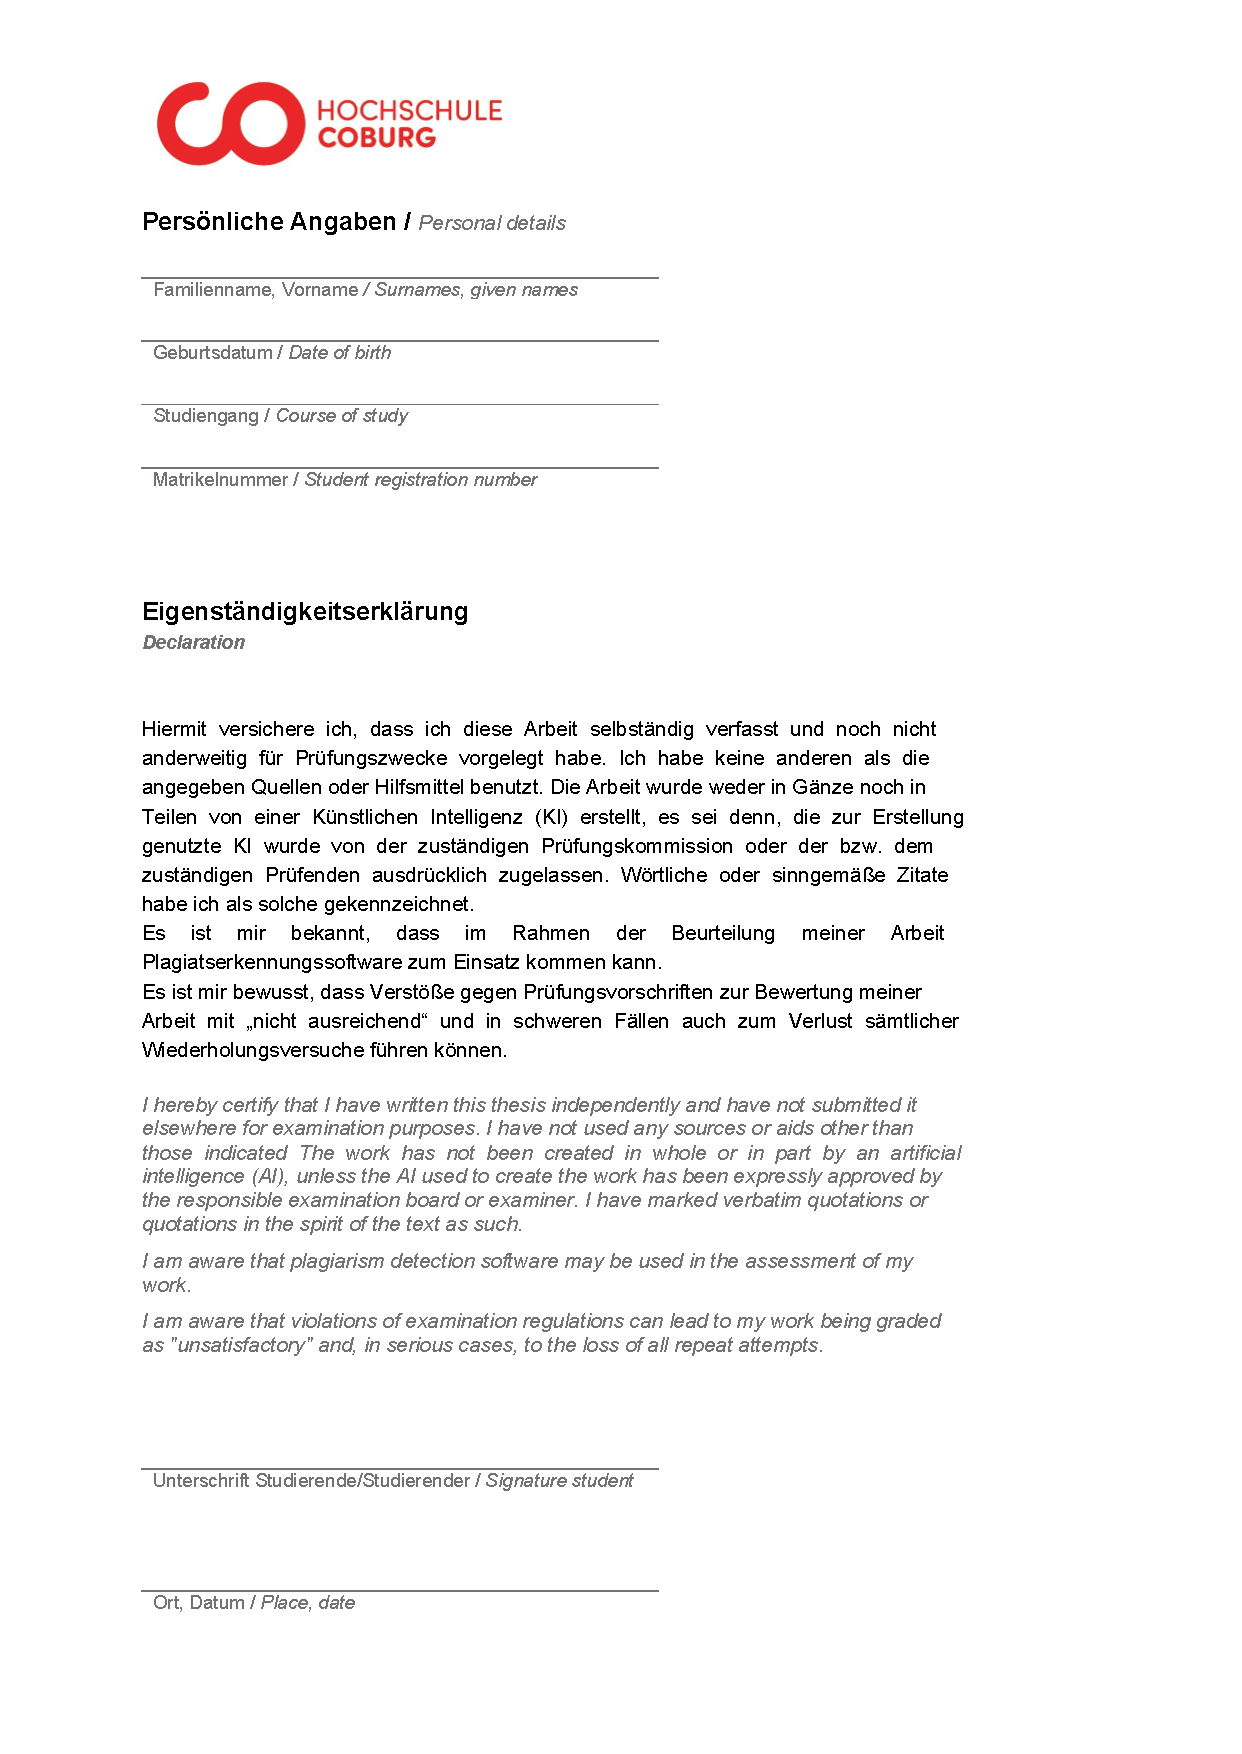
\includepdf[
  pages=-,
  pagecommand={},
  picturecommand*={
    \put(75,714){\large \Autorenname}
    \put(75,683){\large \Geburtsdatum}
    \put(75,652){\large \Studiengang}
    \put(75,622){\large \Matrikelnummer}
    \put(75,81.5){\large \Ort, den \today}
  }
]{framework/_Declaration_of_Honor.pdf}


  % TODO list
  \iftotalcounttodos
    \listoftodos[TODOs]
  \fi

  \end{document}
}

% ===========================================================================
%                   Simplified centered & colored tables
% ===========================================================================

\newenvironment{colortable}[1]{
  \begin{center}
    \begin{tabular}{#1}
    \hline
    \rowcolor{Gray}
}
{
    \hline
    \end{tabular}
  \end{center}
}

\newcommand{\tablecontent}{
  \hline
  \rowcolor{White}
}


\def\Titel{\fontsize{20}{30} \selectfont Entwicklung und Evaluierung einer Spiele-KI für „Ganz schön clever“ mittels Deep Reinforcement Learning}
\def\Dozent{Prof. Dr. Mittag, Florian}

% Infos zum Autor
\def\Autorenname{Schubert, Sander}
\def\Geburtsdatum{02.12.1994}
\def\Matrikelnummer{01550217}
\def\Studiengang{Informatik Bachelor}

% Infos zum Unternehmen
\def\Unternehmen{}
\def\Abteilung{}
\def\Strasse{}
\def\Ort{}

% Infos zum Betreuer
\def\Betreuer{Prof. Dr. Mittag, Florian}
\def\Funktion{Betreuer}
\def\Telefon{+49 (0)9561 317-316}
\def\Email{Florian.Mittag@hs-coburg.de}

% Daten
\def\Beginn{<BEGINN>}
\def\Ende{<ENDE>}
\def\Abgabe{\today}

\startHSCdocument[Bachelorarbeit]

Abb. 1: Ganz schön clever 

Abb. 2: Rundenablauf Ganz schön clever

Abb. 3: Reinforcement Learning

Abb. 4: Zustandsverlauf Ganz schön clever

Abb. 5: Multilayer Perceptron

Abb. 6: Swimlane-Diagramm des Projektes

Abb. 7: Ablauf-Diagramm der Schritt Funktion 1

Abb. 8: Ablauf-Diagramm der Schritt Funktion 2

Abb. 9: Hyperparameter der Künstlichen Intelligenz

Abb. 10: ReLU Funktion

Abb. 11: Erstes erfolgreiches Training

Abb. 12: Erstes erfolgreiches Training 100 Schritte

Abb. 13: Training ohne Aktionsmaske

Abb. 14: Training mit Aktionsmaske

Abb. 15: Ungültige Züge mit zwei Würfeln

Abb. 16: Ungültige Züge mit vier Würfeln

Abb. 17: Optimiertes Training

Abb. 18: Erstes Training mit allen Feldern

Abb. 19: Performance 40000 Schritte

Abb. 20: Ungültige Züge 40000 Schritte

Abb. 21: Performance 4000 Schritte

Abb. 22: Ungültige Züge 4000 Schritte


\include{Verzeichnisse/Abkürzungsverzeichnis}
Code 1: Klassenattribute für Runden

Code 2: Klassenattribute für Würfel

Code 3: Klassenattribute für Punktestand

Code 4: Klassenattribute für farbige Felder

Code 5: Klassenattribute für freizuschaltende Boni

Code 6: Klassenattribute für Punktestand

Code 7: Klassenattribute für Belohnungsflags

Code 8: Klassenattribute für Punktestände der Felder

Code 9: Klassenattribute für freigespielte Boni

Code 10: Klassenattribute für gewählte Kästchen in den farbigen Feldern

Code 11: Klassenattribute Aktionsraum und Beobachtungsraum

Code 12: Schritt Methode

Code 13: Methode zum Zurücksetzen der Umgebung

Code 14: Methode zur Visualisierung der Spielumgebung

Code 15: Würfel Methode

Code 16: Methode zur Überprüfung der freigespielten Belohnungen

Code 17: Methode zur Generierung des Beobachtungsraumes

Code 18: Methode zur Generierung der Aktionsmaske

Code 19: Methode zum Hinzufügen von Boni

Code 20: Methode zum Inkrementieren von Runden

Code 21: Methode zu anlernen des Modells

Code 22: Methode zum Vorhersagen mithilfe des Modells

Code 23: Methode zur Initialisierung der Spielumgebungen

Code 24: Methode zum Anwenden der Aktionsmaske

Code 25: Methoden zum Erstellen von Einträgen

Code 26: Methode zum plotten von Historien

Code 27: Anwendungsbeispiel
\section{Einleitung}
\subsection{Kurzzusammenfassung}
Zunehmend prägen das maschinelle Lernen und KI die Arbeit und das Leben der Menschen. Besonders präsent sind im Jahr 2023 unter Anderem potente Chatbots wie ChatGPT 4. Solche Tools ermöglichen es Benutzern komplexe sowie komplizierte Aufgaben deutlich einfacher und schneller abzuarbeiten. Hervorzuheben ist hierbei auch, dass man mit solchen Tools deutlich weniger Fachwissen benötigt um in einem Bereich aufgaben effizient lösen zu können, da es einem eine Vielzahl von Informationen zum gewünschten Thema auf anfrage bereitstellen kann. Je komplexer das Problem oder die Fragestellung allerdings sind, desto unverlässlicher werden diese Tools. Man muss seine Anfragen deshalb möglichst präzise formulieren und die Problemstellung in für das Tool angemessene Teilaufgaben zerlegen.

Auch in der Spielentwicklung spielen maschinelles Lernen und KI schon seit langem eine bedeutende Rolle. In den meisten Spielen gibt es sogenannte Bots, welche man als KI bezeichnen kann. Diese sollen bestimmte Aufgaben im Spiel erfüllen um den Spieler zu unterstützen oder im als Widersacher zu dienen. Je komplexer die Aufgabe, umso schwerer ist es einen solchen Bot zu erstellen, welcher die Aufgabe auf zufriedenstellende Weise erfüllen kann.

Das Gesellschaftsspiel "Ganz schön clever" ist ein Würfelspiel, welches eine hohe Komplexität aufweist. Diese kommt vor allem durch die vielen Aktionsmöglichkeiten des Spielers und die multiplen zusammenhängen innerhalb des Belohnungssystems zustande. Außerdem weist es eine hohe Stochastizität auf, welche die Komplexität weiter erhöht.
Ziel dieser Arbeit ist es eine KI beziehungsweise einen Bot für dieses Spiel zu entwickeln, der das Spiel effizient spielen kann, sowie zu analysieren welche Aspekte der Entwicklung dabei relevant und zu beachten sind.

Dazu mussten Spielumgebung sowie KI zunächst implementiert werden. Dies geschah mithilfe von Bibliotheken wie Stable-Baselines3 und Gymnasium.
Insgesamt ergab sich dabei, dass sich mithilfe des PPO-Algorithmus von Stable-Balseslines3 auf relativ einfache Weise ein effizientes Modell für das Spiel entwickeln lässt.
\subsection{Hinführung zum Thema}
In den vergangenen Jahren gewann maschinelles Lernen und insbesondere die Künstliche Intelligenz zunehmend an Bedeutung, Tendenz steigend. Im Jahr 2023 ist eines der präsentesten neuen Tools ChatGPT 4. Dieses Tool ist ein Chat-Bot, welcher es dem Benutzer ermöglicht mit ihm zu kommunizieren und ihm Fragen oder Aufgaben zu stellen. Solche Tools ermöglichen es Benutzern zunehmend ihre Tätigkeiten zu vereinfachen und prägen somit das Leben der Menschen zunehmend. Auch in dieser Arbeit wurde ChatGPT 4 als unterstützendes Tool verwendet. Es wurde vor Allem dafür benutzt um fachliche Fragen zu beantworten, aber auch anfangs um Code für den Prototypen zu generieren. Mit zunehmender Komplexität der zu bearbeitenden Aufgabe sinkt die Verlässlichkeit solcher Tools. Daher ist es wichtig die Anfragen an den Chat-Bot möglichst präzise zu formulieren und den Aufgabenbereich angemessen einzuschränken um das Tool nicht zu überfordern.

Auch in der Spielentwicklung nimmt das maschinelle Lernen und die Künstliche Intelligenz schon seit langem eine zentrale Rolle ein. In den meisten Spielen gibt es eine oder mehrere Künstliche Intelligenzen, welche bestimmte Aufgaben erfüllen, um den Spieler bei Spiel zu unterstützen oder ihm als Widersacher zu dienen. Auch hier gilt je komplexer die Aufgabenstellung desto schwieriger ist es einen solchen Bot zu generieren, welcher diese effizient und richtig lösen kann.

Das Gemeinschaftsspiel "Ganz schön clever" ist ein Würfelspiel, welches eine hohe Komplexität aufweist. Diese kommt vor allem durch die hohe Anzahl an möglichen Aktionen (dem sogenannte Aktionsraum) für den Spieler und die vielen Zusammenhänge des Belohnungssystems im Spiel zu Stande. Das Spiel weist zusätzlich eine hohe Stochastizität auf, welche die Komplexität weiter erhöht.

Interessant ist wie man für ein solch komplexes Spiel einen Bot oder eine Künstliche Intelligenz entwickeln kann um dieses effizient spielen zu können. Ist die Komplexität möglicherweise zu groß, um vom Bot erfasst zu werden und wenn nicht, wie kann man einen solchen Bot implementieren und was gilt es dabei zu beachten?
\subsection{Zielsetzung und Motivation}
Ziel der Arbeit ist es einen Bot beziehungsweise eine Künstliche Intelligenz zu entwickeln, welche das Spiel "Ganz schön clever" möglichst effizient spielen kann. Dabei soll analysiert werden, welche Aspekte es dabei zu beachten gilt und wie sich unterschiedliche Ansätze auf das Verhalten und die Performance des Modells (des Bots) auswirken.

In den vergangenen Jahren hat sich viel getan, weshalb deutlich mehr möglich geworden ist. Mit neuen Möglichkeiten ergeben sich auch bessere oder einfachere Ansätze, die zu einem wünschenswerten Ergebnis führen. Ziel ist es auch einen geeigneten Ansatz zu finden und zu vervollständigen.

Es gibt des Weiteren noch keine Untersuchungen zu einer Spiel-KI für das Spiel "Ganz schön clever" daher ist es interessant Erkenntnisse darüber zu gewinnen welche Schwierigkeiten sich hierbei ergeben und wie man diese überwinden kann.
\subsection{Aufgabenstellung}
Es ist eine KI für das Spiel "Ganz schön clever" zu implementieren. Hierbei sollen der Vorgang sowie Ergebnisse des Prozesses analysiert und bewertet werden. Hierzu wird zunächst ein Prototyp entwickelt, welcher eines der fünf Felder des Spiels beinhaltet. Dieser soll Einsichten über die Machbarkeit und die Rahmenbedingungen des Projektes geben. Daraufhin werden das Modell und die Spielumgebung schrittweise um ihre jeweiligen Funktionalitäten erweitert, bis das Spiel vollständig und möglichst effizient von der Künstlichen Intelligenz gespielt werden kann.
\subsection{Aufbau der Arbeit}
Die Arbeit beginnt mit einem Grundlagenteil, bei dem zunächst das Spiel Ganz schön clever und seine Mechaniken erklärt werden. Anschließend werden Maschinelles Lernen, Reinforcement Learning, Deep Learning und Proximal Policy Optimization behandelt, um eine Grundlage für das Verständnis der Abläuft beim Training der Künstlichen Intelligenz zu bieten. Im folgenden werden die verwendeten Technologien des Projektes behandelt. Die vorgestellten Technologien sind Gynmansium, Stable Baselines 3, Matplotlib und ChatGPT 4.

Das nächste Kapitel befasst sich mit den Anforderungen und der Konzeption des Projektes. Es werden Rahmenbedingungen des Projektes sowie die Anforderungen und die Konzeption für die Spielumgebung und die Künstliche Intelligenz besprochen.

Das nächste Kapitel zeigt und erklärt die Implementierung des Projektes. Dabei werden die Variablen und Methoden des Projektes erläutert und beschrieben. Zum einem großen Teil wird Pseudocode verwendet, um die Implementierung verständlicher zu machen und den Umfang zu begrenzen.

Das letzte Kapitel befasst sich mit den Ergebnissen des Projektes. Zunächst wird der Implementierungsverlauf behandelt. Es wurde ein Prototyp erstellt und dieser wurde dann Stück für Stück erweitert. Daraufhin folgen die Analyse und zur Schau Stellung des finalen Modells.

Zum Abschluss folgt eine Zusammenfassung und Anreize zur Weiterarbeit am Projekt.
\subsection{Erläuterungen zur Lesbarkeit der Arbeit}
Es gilt zu beachten, dass viele der Abbildungen innerhalb der Arbeit nicht selbsterklärend sind und es wichtig ist, den anliegenden Text zu lesen, um sie ordentlich verstehen zu können. 

Es wird häufig von "Kästchen" und "Feldern" gesprochen. Ein "Kästchen" ist ein spezifisches Element auf dem Spielbrett, welches ausgefüllt werden kann, sobald bestimmte Konditionen erreicht sind, wobei sich "Feld" auf die Gesamtheit von "Kästchen" einer bestimmten Farbe bezieht.

Es wird häufig von "Wahlen" gesprochen. Eine "Wahl" beschreibt das Auswählen eines Würfels oder einer Boni zum Ausfüllen eines Kästchens auf dem Spielbrett.

Außerdem wird des öfteren von "Extra Wahlen" und "normalen Wahlen" gesprochen. Innerhalb des Spiels gibt es verschiedene Möglichkeiten Kästchen auszufüllen. Normal durch die Wahl eines Würfels nach einem eigenen Wurf. Mit der Wahl eines Würfels von Silbertablett des Gegners. Mit der Wahl eines Würfels mithilfe des Extra Wahl Boni und durch das Nutzen eines der anderen Boni, welches es erlauben ein Kästchen in einem der Kästchen des Spiels auszufüllen. "Extra Wahlen" beziehen sich hierbei auf Wahlen mithilfe des Extra Wahl Boni oder vom Silbertablett des Gegners, wobei sich "normale Wahlen" auf Wahlen nach dem eigenen Wurf oder mithilfe eines der anderen Boni beziehen.

Es wird im Rahmen des Arbeit auch von "Bonusrunden" gesprochen. Diese beziehen sich auf Wahlen mithilfe von Boni bei "normalen Wahlen"

Des weiteren werden häufig die Begriffe Modell, Agent und Künstliche Intelligenz in einem ähnlichen Zusammenhang verwendet. Ein Modell bezieht sich auf die Entität, welche vorhersagen treffen kann, wenn sie Zustände als Input bekommt. Ein Agent ist die Entität, welche seine Umgebung wahrnimmt und Anhand dieser eine Aktion wählt und ausführt und die Künstliche Intelligenz bezieht sich auf eine Entität, welche eigenständig in einer sich ändernden Umgebung lernen und sich entwickeln kann. Ein Modell ist im Rahmen dieser Arbeit ein Neuronales Netz, welches gelernt hat in bestimmten Zuständen bestimmte Aktionen vorherzusagen. Alle drei Begriffe beziehen sich in der Arbeit im Prinzip auf das selbe Konzept, allerdings setzen die Begriffe verschiedene Schwerpunkte für die Betrachtung des Konzeptes.

Es wird auch häufig von "gültigen Aktionen" oder "gültigen Würfeln" gesprochen. "Gültige Aktionen" sind Aktionen, welche vom Spielablauf vorhergesehen sind. "Gültige Würfel" hingegen beschreiben Würfel, welche zur Wahl stehen und bei einem Wurf geworfen werden dürfen.
\section{Grundlagen}
\subsection{Allgemeine Grundlagen}
\subsubsection{Ganz schön clever}
\begin{minipage}{\linewidth}
	Die folgende Abbildung zeigt das Spielbrett des Spiels "Ganz schön clever" zu dem im Rahmen dieser Arbeit eine KI implementiert werden soll:

	\vspace{0.5cm}
	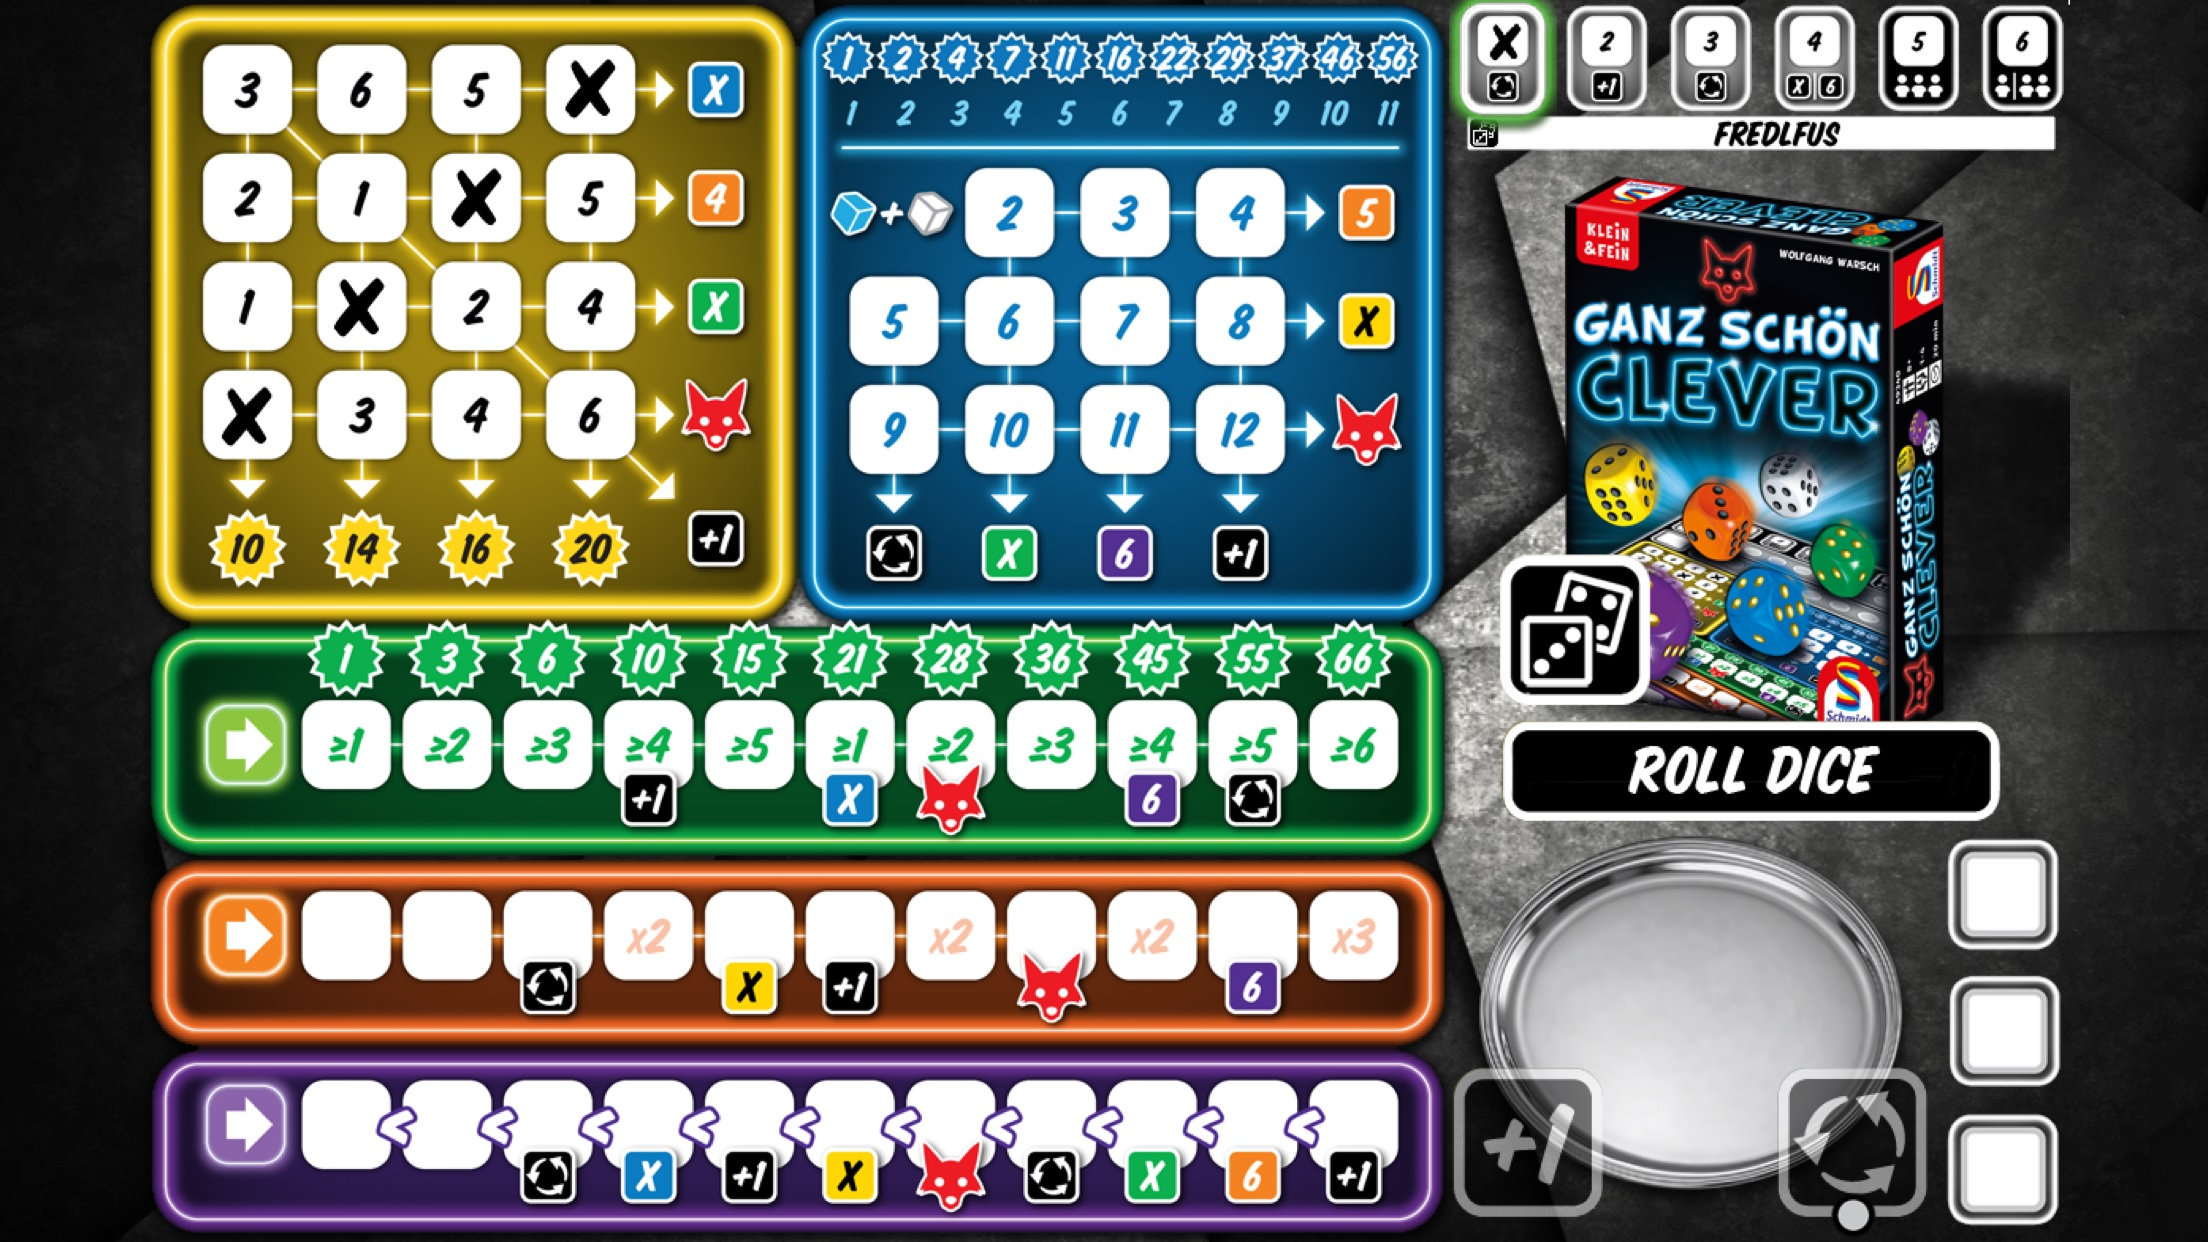
\includegraphics[width=1\textwidth]{Bilder/gsc} 
	
	Abb. 1: Ganz schön clever 
	
	Quelle: [Screenshot des Android Handyspiels Ganz schön clever]\\
\end{minipage}

Im folgenden werden der Spielablauf und die wesentlichen Regeln des Spiels erklärt.

Es gibt sechs farbige Würfel, wobei jeder bis auf den weißen einem der 5 farbigen Spielfelder zuzuordnen ist. Der weiße Würfel ist ein Sonderwürfel und kann als einer der anderen Würfel betrachtet werden. Wenn bestimmte Bedingungen erfüllt sind kann der Spieler einen Würfel wählen und das entsprechende Kästchen ausfüllen. Die Felder verfügen über Belohnungen, welche freigeschaltet werden, wenn eine bestimmte Kombination oder Anzahl an Feldern freigeschaltet worden ist. Beim orangenen und lila Feld kommt es bei der Belohnung zudem darauf an wie hoch das Würfelergebnis des gewählten Würfels ist, da die einzelnen Kästchen hier je nach Würfelergebnis zusätzlich belohnt werden.
\\
Das Spiel teilt sich in bis zu sechs Runden mit jeweils bis zu drei Würfen ein. Nach jeder Runde bekommt der Spieler zudem die Möglichkeit einen Würfel auf dem Silbertablett eines Mitspielers zu wählen. Diese Wahl verhält sich so wie bei der Wahl eines eigenen Würfels bei den Würfen des Spielers selbst. Die Anzahl der Runden werden von der Spielerzahl festgelegt. Bei ein bis zwei Spielern sind es sechs Runden. Bei drei Spielern sind es fünf Runden und bei vier Spielern sind es vier Runden. Die Anzahl der Würfe pro Runde ist immer drei, allerdings kann diese Anzahl reduziert werden, wenn kein Würfel mehr zum Würfeln zur Verfügung steht. Dann wird der Spielablauf fortgesetzt als hätte der Spieler seinen dritten Wurf in der Runde beendet und er kann einen Würfel vom Tablett des Mitspielers wählen bevor dann die neue Runde für ihn beginnt. Zu beginn der ersten, zweiten, dritten und vierten Runde bekommt jeder Spieler zudem eine Belohnung, welche oben rechts auf Abbildung 1 bei der jeweiligen Rundenzahl zu sehen ist. Die Belohnung in Runde vier steht dabei für das freie ausfüllen eines beliebigen Kästchens mit dem jeweils maximal möglichen Wert für das Kästchen.
\\
Es gibt zwei Arten von Belohnungen im Spiel. Punktebelohnungen und Boni. Bei Punktebelohnungen handelt es sich um Punkte welche auf den Score des Spielers addiert werden, welcher am Ende des Spiels entscheidet wer gewonnen hat. Der Spieler mit dem höchsten Score gewinnt das Spiel. Punktebelohnungen erhält man beim gelben Feld indem man eine Spalte vollständig ausfüllt. Die Anzahl der Punkte findet sich am Ende der Spalte. Im blauen Feld erhält man Punktebelohnungen mit zunehmender Anzahl an ausgefüllten blauen Kästchen. Die Anzahl der Punkte findet sich im oberen Bereich des blauen Feldes. Im grünen Feld ebenso mit zunehmender Anzahl der ausgefüllten grünen Kästchen. Die Anzahl der Punkte findet sich auch hier im oberen Bereich des grünen Feldes. Im orangenen und lila Feld muss man für Punktebelohnungen lediglich ein Kästchen ausfüllen. Die Punktebelohnung entspricht der Augenzahl des entsprechenden ausgefüllten Kästchens. Beim orangenen Feld wird diese Augenzahl bei einigen Feldern zusätzlich mit zwei oder drei multipliziert. Außerdem gibt es eine Boni Belohnung, welche indirekt eine Punktebelohnung darstellt. Es handelt sich hierbei um den sogenannten Fuchs beziehungsweise die Füchse. Die Anzahl der freigeschalteten Füchse wird am Ende des Spiels mit der Anzahl der erzielten Punkte des Feldes mit den niedrigsten erreichten Punktewert multipliziert und zum Gesamtpunktestand addiert.

Bei Boni handelt es sich um Belohnungen, welche der Spieler nutzen kann oder muss, um sich im Spiel einen Vorteil zu verschaffen. Die Boni sind bei den entsprechenden Kästchen beziehungsweise am Rande von Spalten und Zeilen eingezeichnet und können freigeschaltet werden indem man diese (Kästchen beziehungsweise Zeilen oder Spalten) ausfüllt. Eine Ausnahme bildet hier die Boni welche beim gelben Feld freigeschaltet wird indem alle diagonalen Felder von links oben nach rechts unten ausgefüllt werden. \\

Jede Boni hat ihr eigenes Symbol. Nun folgt eine Aufzählung und Erklärung der verschiedenen Boni mit Ausnahme der Füchse. Boni werden bei der Benutzung aufbraucht. Man kann mehr als eine dieser Boni auf einmal besitzen. Die Boni sind stapelbar.

Extra Wahl: Bei der Extra Wahl wird es dem Spieler ermöglicht am Ende seiner eignen Runde beziehungsweise nachdem er einen Würfel vom Silbertablett des Gegners gewählt hat erneut Würfel zu wählen und die entsprechenden Kästchen dafür anzukreuzen. Würfel die so gewählt wurden können mithilfe der Extra Wahl Boni nicht erneut gewählt werden solange keine neue Runde oder Wahl vom Silbertablett beginnt. Mit der Extra Wahl Boni können alle Würfel gewählt werden, nicht nur die, welche unter normalen Umständen gültig zur Wahl stehen würden. Das Symbol ist die +1.

Neuer Wurf: Der Neue Wurf ermöglicht es dem Spieler einen seinen Würfe zu wiederholen ohne dabei einen der Würfel auszuwählen. Dies ermöglicht es ihm Würfe mit ungünstigen Ergebnissen neu auszurichten. Das Symbol sind die drei Pfeile, welche im Kreis angeordnet sind.

Gelbes Kreuz: Ermöglicht es dem Spieler direkt nach erhalten der Boni eines der gelben Kästchen nach eigener Wahl auszufüllen. Das Symbol ist ein Kreuz auf gelbem Hintergrund.

Blaues Kreuz: Ermöglicht es dem Spieler direkt nach erhalten der Boni eines der blauen Kästchen nach eigener Wahl auszufüllen. Das Symbol ist ein Kreuz auf blauem Hintergrund.

Grünes Kreuz: Ermöglicht es dem Spieler direkt nach erhalten der Boni das nächste freie Grüne Kästchen auszufüllen. Das Symbol ist ein Kreuz auf grünem Hintergrund.

Orangene Vier: Ermöglicht es dem Spieler direkt nach erhalten der Boni das nächste freie orangene Kästchen mit einer vier auszufüllen. Das Symbol ist eine vier auf orangenem Hintergrund.

Orangene Fünf: Ermöglicht es dem Spieler direkt nach erhalten der Boni das nächste freie orangene Kästchen mit einer fünf auszufüllen. Das Symbol ist eine fünf auf orangenem Hintergrund.

Orangene Sechs: Ermöglicht es dem Spieler direkt nach erhalten der Boni das nächste freie orangene Kästchen mit einer sechs auszufüllen. Das Symbol ist eine sechs auf orangenem Hintergrund.

Lila Sechs: Ermöglicht es dem Spieler direkt nach erhalten der Boni das nächste freie lila Kästchen mit einer sechs auszufüllen. Das Symbol ist eine sechs auf lila Hintergrund. \\

Nun folgen die Regeln nach denen bestimmt wird ob ein Würfel gewählt werden kann, um ein Kästchen auszufüllen und um zu bestimmen ob er ein gültiger Würfel ist:

Ist ein Würfel ungültig kann dieser nicht gewählt werden. Würfel werden ungültig indem sie in der aktuellen Runde oder bei einer Wahl mit dem Extra Wahl Boni bereits gewählt worden sind. Außerdem werden Würfel, welche eine geringere Augenzahl aufweisen als der aktuell gewählte Würfel automatisch ungültig. Eine Ausnahme ist hierbei die Wahl eines Würfels vom Silbertablett des Gegenspieler oder Wahlen von Würfeln durch die Extra Wahl Boni. Würfel werden wieder gültig am Anfang jeder neuen Runde, nach Abschluss des dritten Wurfes, sowie nach der Wahl des Würfels vom Silbertablett, als auch nachdem Wahlen mit dem Extra Wahl Boni erfolgt sind. Dabei bleiben mithilfe der Extra Wahl Boni gewählte Würfel solange ungültig, bis keine weiteren Extra Wahl Boni in diesem Spielschritt mehr verwendet werden und das Spiel normal weiter geht.

Jedes Feld hat seine eigenen Regeln, die bestimmen, wann ein Kästchen ausgefüllt werden darf. Beim gelben Feld muss die Augenzahl des Würfel mit der Zahl des Kästchens übereinstimmen. Beim Blauen Feld muss die Summe der Augenzahlen des blauen und des weißen Würfels mit der Zahl innerhalb des Kästchens übereinstimmen. Beim grünen Feld muss die Augenzahl des Würfels größer oder gleich der Zahl im Kästchen sein. Zudem kann beim grünen Feld immer nur das nächste freie Kästchen ausgefüllt werden, beginnend von links. Im orangenen Feld kann immer das nächste Kästchen eingetragen werden. Auch hier beginnend von links. Beim lila Feld muss die Augenzahl des Würfels größer sein als die Zahl im zuletzt ausgefüllten Kästchen. Eine Ausnahme bildet hier der Fall in dem eine sechs im zuletzt ausgefüllten Kästchen steht. Dann kann das nächste Feld mit jeder beliebigen Augenzahl gewählt werden. Die sechs setzt die Voraussetzung für das lila Feld bis zum nächsten ausfüllen im lila Feld aus. Auch hier gilt die Reihenfolge von links nach rechts.
\subsubsection{Maschinelles Lernen}
"Maschinelles Lernen heißt, Computer so zu programmieren, dass ein bestimmtes Leistungsmerkmal anhand von Beispieldaten oder Erfahrungswerten optimiert wird" [Maschinelles Lernen, Seite 3].

Es gibt bis heute nach wie vor viele Problemstellungen, die von Menschen auf einfache Art und weise lösbar sind, für die es aber keine algorithmische Lösung zu geben scheint. Hier kommt das maschinelle Lernen zum Einsatz. Durch die Mustererkennung aus Trainingsdaten können Programme lernen solche Problemstellungen zu lösen indem sie präzise Vorhersagen über bestehende Sachverhalte beziehungsweise Muster aus beliebigen Daten des selben oder eines ähnlichen Sachverhaltes, der beim generieren der Trainingsdaten vorhanden war, zu treffen. Ein besonders weit verbreiteter Anwendungsfall ist die Herleitung von Kundenverhalten und möglicher Optimierungsmöglichkeiten für den Verkauf. Wenn man ein Programm verwendet, um eine Struktur mithilfe von maschinellem Lernen zu trainieren, damit diese Vorhersagen über ähnliche Sachverhalte treffen kann, nennt man diese dann Modell. Ein solches Modell wird häufig erst auf allgemeinen Datensätzen und später auf immer spezifischeren Daten trainiert, sodass es schließlich auf eine konkrete Aufgabe zugeschnitten werden kann [Maschinelles Lernen, Seite 1f].

Maschinelles Lernen ermöglicht es zwar nicht einen gesamten Prozess mit all seinen Einzelheiten zu verstehen, aber es ermöglicht relevante Merkmale zu erkennen und mithilfe dieser Merkmale und deren Zusammenhängen Prognosen über einen gesamten Sachverhalt herzuleiten. Auf Grund dieser Prognosen kann schließlich agiert werden. [ML, Seite 2].

Die Anwendungsgebiete von maschinellem Lernen sind zahlreich. Unter anderem ist es relevant für den Einzelhandel und Finanzdienstleister, um Kreditgeschäfte abzuwickeln, Betrugsversuche zu erkennen, oder den Aktienmarkt einzuschätzen. Aber auch in der Fertigung wird es zur Optimierung, Steuerung und Fehlerbehebung eingesetzt. Auch in der Medizin erweisen sich medizinische Diagnoseprogramme mithilfe von Modellen, die mit maschinellem Lernen trainiert wurden als nützlich [ML, Seite 3].

Und das sind nur einige wenige der zahlreichen möglichen Bereiche in denen maschinelles Lernen bereits Anwendung findet. 

Die Datenbestände und das World Wide Web werden immer größer und die Suche nach relevanten Daten kann nicht mehr manuell vorgenommen werden [ML, Seite 3].

"Das maschinelle Lernen ist aber nicht nur für Datenbanken relevant, sondern auch für das Gebiet der künstlichen Intelligenz" [ML, Seite 3].

Von Intelligenz spricht man dann, wenn das System selbstständig in einer sich verändernden Umgebung lernen und sich anpassen kann. Dadurch muss der Systementwickler nicht jede erdenkliche Situation vorhersehen und passende Lösungen dafür entwickeln [ML, Seite 3].
 
Maschinelles Lernen findet seine Anwendung in dieser Arbeit in Form von Deep Reinforcement Learning. Was Reinforcement Learning ist und wie es sich von Deep Reinforcement Learning unterscheidet wird im Folgenden beschrieben.
\subsubsection{Reinforcement Learning}
Reinforcement Learning (im deutschen: bestärkendes Lernen) heißt so, weil es die Aktionen des Agenten (beziehungsweise des Modells) bestärkt. Man kann sich das in etwa so vorstellen, wie das Training eines Hundes im Park. Dieser wird jedes mal wenn er einen Trick richtig ausführt mit einem Leckerli belohnt. Diese Belohnung bestärkt das Verhalten des Hundes und das Tier lernt dieses in Zukunft zu wiederholen. Eine negative Aktion kann hingegen bestraft werden, damit sie in Zukunft nicht wiederholt wird [RL, Seite 11].

Im Reinforcement Learning sind vor allem Folgende Begriffe wichtig:

Agent (oder Modell): Dabei handelt es sich um die Entität, welche mit der Umgebung interagiert und die Entscheidungen trifft. Dabei kann es sich zum Beispiel um einen Roboter oder autonomes Fahrzeug handeln [RL, Seite 11]. In dieser Arbeit ist diese Entität ein Modell, welches mithilfe der Bibliothek Stable-Baselines3 erstellt wird.

Umgebung: Dabei handelt es sich um die Außenwelt des Agenten [RL, Seite 11]. der Agent interagiert mit dieser und erhält je nach Zustand der Umgebung und seiner gewählten Aktion ein entsprechendes Feedback.

Aktion: Eine Aktion beschreibt das Verhalten des Agenten [RL, Seite 11]. In dieser Arbeit wählt der Agent Kästchen des Spielbrettes aus, um diese auszufüllen. Außerdem entscheidet er ob er bestimmte Boni zu einem gegebenen Zeitpunkt nutzen möchte oder nicht.

Zustand: Der Zustand beschreibt den Zusammenhang zwischen Umgebung und Agent [RL, Seite 11]. In dieser Arbeit ist der Zustand von den Eigenschaften des Spielbrettes, der Würfel, der Rundenanzahl und der erspielten Boni abhängig.

Belohnung: Positive oder negative Vergeltung je nachdem wie gut der Zustandswechsel von Zustand x nach Zustand y gewesen ist [RL, Seite 11]. In dieser Arbeit wird dies durch die jeweiligen Punktebelohnungen im Spiel verkörpert. Eine Ausnahme bildet hier eine negative Belohnung, wenn der Agent in einen Zustand gerät in dem er keine gültige Aktion tätigen kann.

Policy: Die Policy ist die Strategie des Agenten, nach welcher er seine nächsten Aktionen wählt [RL, Seite 11]. In dieser Arbeit wird die Policy durch ein Multilayer Perceptron (siehe Deep Learning) abgebildet.

Episode: Eine Menge an Zusammenhängenden Aktionen, welche endet, wenn das Ziel erreicht worden ist [RL, Seite 11]. In dieser Arbeit ist eine Episode ein kompletter Spieldurchlauf von Ganz schön clever.

\begin{minipage}{\linewidth}
	Die folgende Abbildung beschreibt einen Lernzyklus im Reinforcement Learning:

	\vspace{0.5cm}
	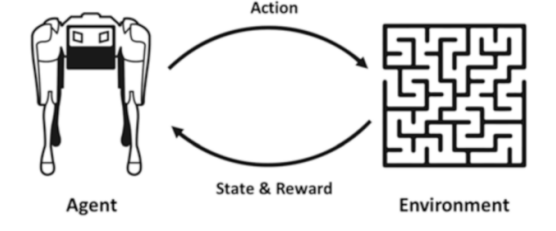
\includegraphics[width=0.8\textwidth]{Bilder/rl}
	
	Abb. 2: Reinforcement Learning
	
	Quelle: [RL, Seite 12]\\
\end{minipage}

Der Agent führt eine Aktion in der Umgebung aus und erhält daraufhin eine Belohnung und den neuen Zustand der Umgebung als Feedback. Daraufhin aktualisiert er seine Policy, um in Zukunft bessere Aktionen tätigen zu können.

Hierbei ist das Ziel des Agenten die gesamte erreichte Belohnung zu maximieren. Demnach wird die Policy dementsprechend angepasst, dass dies begünstigt wird [RL, Seite 12f].

Doch dabei gibt es einige Schwierigkeiten, die es zu beachten gilt. Belohnungen die in kurzer Zeit erreicht werden können, könnten wichtiger oder weniger wichtig sein als Belohnungen, die erst innerhalb vieler Schritte erreicht werden können. Ein gutes Beispiel hierfür wäre ein Balanceakt, bei dem es besonders wichtig ist kurzzeitige Belohnungen zu bevorzugen, da die Episode endet, wenn das Balancieren fehlschlägt, was eine starke negative Belohnung zur Folge haben kann.

Ein weiterer Faktor ist die Balance zwischen Erkundung und Ausbeutung. Diese zwei Prinzipien sind wesentlich für das Reinforcement Learning. Dabei geht es darum, wie stark die Policy es vorzieht neue oder selten gesehene Zustände und Aktionen auszuprobieren oder bereits bekannte, welche eine gute Belohnung zu bringen scheinen auszunutzen beziehungsweise auszubeuten [RL, Seite 13].
\subsubsection{Deep Learning}
Was unterscheidet Reinforcement Learning von Deep Reinforcement Learning? Im wesentlichen handelt es sich um das selbe Konzept, allerdings ist das eine Deep Learning und das andere nicht. Was ist also Deep Learning?

Von Deep Learning spricht man sobald ein Neuronales Netz mehrere versteckten Schichten hat. 

Ein solches Netz besteht aus einer Vielzahl von Neuronen. [DRL, Seite 75] Ein solches Neuron setzt sich zusammen aus Inputs, Outputs, Gewichtungen dieser In- und Outputs, sowie einer Aktivierungsfunktion, welche auch gewichtet sein kann. Ein Spezialfall eines solchen Neuronalen Netzes ist ein sogenanntes Multilayer Perceptron. Bei diesem sind alle Neuronen in einer Schicht mit allen Neuronen der folgenden Schicht verbunden. Häufig haben auch alle Neuronen der versteckten Schichten die selbe Aktivierungsfunktion. Was den Beitrag der einzelnen Neuronen zum Gesamtergebnis des Netzes steuert sind im wesentlichen seine Gewichtungen und die Position im Netz.

\begin{minipage}{\linewidth}
	Die folgende Abbildung zeigt ein solches Multilayer Perceptron. Dabei sind nicht alle Verbindungen eingezeichnet, um Übersichtlichkeit zu gewährleisten:
	
	\vspace{0.5cm}
	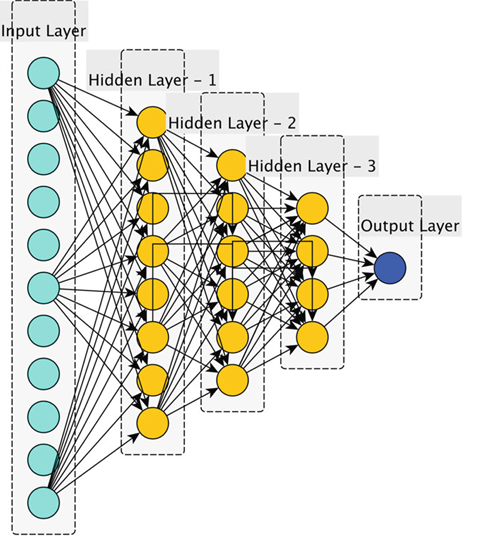
\includegraphics[width=0.8\textwidth]{Bilder/mlp} 
	
	Abb. 3: Multilayer Perceptron
	
	Quelle: [DRL, Seite 78]\\
\end{minipage}


Die Inputs des Netzes sind die Werte von Variablen der zur Verfügung stehenden Beobachtungen der Umgebung. Die versteckten Schichten verarbeiten diese Inputs dann mit ihren Funktionen und Gewichtungen. Das Output des Netzes ist hingehen eine gewünschte Vorhersage, die mit ihrer eigenen Aktivierungsfunktion hergeleitet wird.
\subsubsection{Proximal Policy Optimization}
Proximal Policy Optimization oder kurz PPO ist eine neue Policy Gradient Methode für Reinforcement Learning. Im Gegensatz zu standardmäßigen Policy Gradient Methoden ist es mit dieser Methode möglich mehrere Policy Updates pro Datenpaket durchzuführen. PPO hat einige der Vorteile der Trusted Region Policy Optimization (kurz TRPO), ist aber simpler zu implementieren und hat auch andere Vorteile, wie bessere Generalisierbarkeit und niedrigere Stichproben Komplexität. PPO zeigt eine gute Balance zwischen Stichproben Komplexität, Einfachheit und Trainingsgeschwindigkeit [PPO, Seite 1].

Die Stichprobenkomplexität beschreibt wie groß ein Datenpaket sein muss, um dem Algorithmus ein gewisses Level an Performanz zu ermöglichen. Dies ermöglicht es mehr Updates mit weniger Gesamtdaten durchzuführen, was vor allem hilfreich ist, wenn nicht genügend Daten zur Verfügung stehen oder diese nur schwer zu generieren sind.

Policy Gradient Methoden berechnen einen Gradienten und passen die Policy in Richtung der negativen Steigung an. Das kann man sich ähnlich wie einen Punkt auf einer Parabel vorstellen, die Policy entspricht dem Punkt und wird so lange angepasst beziehungsweise verschoben, bis sie möglichst das Minimum der Parabel erreicht. Dieses Minimum spiegelt eine optimale Policy wieder.

Bei der Trusted Region Policy Optimization gibt es eine vertrauenswürdige Region innerhalb derer die Policy abgeändert werden darf. Das soll sicherstellen, dass die Policy nicht zu stark abgeändert wird, um ein stabileres Training zu gewährleisten. Im Gegensatz zur PPO werden Änderungen, die zu stark abweichen verworfen.

Bei der PPO kommt es zum sogenannten Clipping. Hierbei werden zu starke Änderungen im übertragenen Sinne abgeschnitten und es kommt zu einer abgeschwächten Änderung der Policy.

PPO ist ein verhältnismäßig simpler, einfach zu verstehender und dennoch effizienter Algorithmus. Er hat eine gute Balance zwischen Stabilität und Effizienz. Außerdem erzielt er gute Ergebnisse bei einer großen Bandbreite an Aufgaben. Daher eignet sich PPO besonders gut für Einsteiger, die bisher nicht viel mit Deep Reinforcement Learning gearbeitet haben.
\subsection{Verwendete Technologien}
\subsubsection{Gymnasium}
Gymnasium ist die Fortführung der OpenAi Bibliothek Gym [Gym]. Sie kann genutzt werden, um Umgebungen zu schaffen, die für maschinelles Lernen verwendet werden können. Die Bibliothek bietet auch eine Menge vordefinierter Umgebungen, welche kostenfrei genutzt werden können, was gerade für Einsteiger den Vorteil hat sich mit wenig Aufwand ausprobieren zu können.

Die Bibliothek bietet Kernmethoden, welche später selbst gefüllt und implementiert werden müssen, um die Bibliothek mit einer benutzerdefinierten Umgebung nutzen zu können. Die wesentlichen Methoden, welche auf jeden Fall implementiert werden müssen sind die Schritt-Methode (im Englischen step-method) und eine Methode zum zurücksetzen der Umgebung auf den Startzustand (im Englischen reset-method). Außerdem muss eine Initialisierung der Umgebungsklasse erfolgen. Die Schritt-Methode nimmt eine Aktion entgegen und führt diese in der Umgebung aus. Außerdem liefert sie den Zustand der Umgebung nach dem Ausführen der Aktion und die Belohnung für den ausgeführten Schritt zurück. Die Reset-Methode setzt alle relevante Werte der Umgebung auf den Ausgangswert zurück, sodass das Spiel oder die Aufgabe von vorne gestartet werden kann. Des Weiteren bietet es sich an eine Methode zu implementieren, welche den aktuellen Zustand der Umgebung zurückgibt, dies ist allerdings optional.

Gymnasium bietet eine gute Anbindung an die Bibliothek Stable Baselines 3, welche Methoden zum Trainieren eines Modells auf Basis einer eben solchen Gymnasium Umgebung bietet. In dieser Arbeit wird Gymnasium für die Implementierung der Spielumgebung von Ganz schön clever verwendet, damit diese anschließend mithilfe von Stable Baselines 3 trainiert werden kann.
\subsubsection{Stable Baselines 3}
"Stable Baselines 3 ist eine Bibliothek, welche verlässliche Implementierungen von Reinforcement Learning Algorithmen in Pytorch bietet" [SB3, Seite 1]. 

Die Algorithmen haben ein konsistentes Interface und eine umfangreiche Dokumentation, was es einfach macht verschiedene Reinforcement Learning Algorithmen zu testen. Die Implementierung bietet eine simple API. Modelle können in nur wenigen Codezeilen trainiert werden. Die Implementierung weist zudem eine hohe Qualität auf. Es gibt auch eine experimentelle Version der Bibliothek, welche Stable Baseline 3 Contributing genannt wird [SB3, Seite 1-3].

In diese Arbeit wird vor Allem der MaskablePPO Algorithmus aus eben dieser Contributing Bibliothek benutzt. Dabei handelt es sich, um eine Erweiterung des PPO Algorithmus von Stable Baseline 3. Dieser MaskablePPO erweitert den PPO Algorithmus um die Funktionalität einer Maskierung. Diese Maskierung ermöglicht es die Wahlwahrscheinlichkeit bestimmter Aktionen auf Null zu setzen. Die Maskierung wurde in der Arbeit verwendet, um ungültige Aktionen auszuschließen, sodass das Modell nicht auf andere Weise lernen muss, diese zu vermeiden. Dies ist ein simpler und effizienter Weg, um zu gewährleisten, dass beim Training keine ungültigen Aktionen gewählt werden.
\subsubsection{Pytorch}
Pytorch ist eines der beiden am weitesten verbreiteten Deep Learning Frameworks. Es bietet die Möglichkeit vereinfacht eigene Deep Learning Algorithmen zu implementieren. Dies erfolgt vor allem mit sogenannten Tensoren. Dabei handelt es sich um mehrdimensionale Matrizen, mithilfe derer die Berechnungen vorgenommen werden. 

Pytorch wurde in dieser Arbeit indirekt verwendet, da Stable Baselines 3 auf Pytorch basiert.
\subsubsection{Matplotlib}
Matplotlib ist eine umfangreiche und mächtige Bibliothek zum Plotten von Daten. In dieser Arbeit wird Matplotlib dafür verwendet, um die erreichten Punkte und ungültigen Züge zu visualisieren.
\subsubsection{ChatGPT 4}
ChatGPT 4 ist die neueste Version eines neuartigen Chat-Bots. Dieser ermöglicht es dem Benutzer Fragen zu stellen oder aussagen zu treffen, auf die er dann eine Antwort bekommt. Die Erzeugnisse des Chat-Bots sind so gut, dass er sich gut eignet, um bei der Konzeption und Programmierung der Arbeit zu unterstützen. Daher wird ChatGPT 4 in dieser Arbeit zum Teil als Hilfestellung bei Unklarheiten zur Funktionsweise von Technologien und beim Bau des Prototypen verwendet. 

Zudem wird im Rahmen der Arbeit analysiert wie gut sich ChatGPT 4 als unterstützendes Werkzeug eignet und welche Vor- und Nachteile, sowie welche Einschränkungen die Nutzung mit sich bringt.
\section{Anforderungen und Konzeption}
\subsection{Anforderungen}
Dieses Kapitel beschreibt die Anforderungen an das Projekt. Das Projekt ist hierbei die Implementierung und die Analyse einer Spiel-KI für das Spiel Ganz schön clever von Anfang bis Ende.
\subsubsection{Rahmenbedingungen}
Der zeitliche Rahmen der Arbeit beträgt vier Monate. In dieser Zeit ist zunächst ein Grundkonzept in Form eines Exposés vorzustellen. Anschließend soll dieses Konzept weiter verfeinert und validiert werden, was schließlich zur Vervollständigung des Projektes mit den gewünschten, sich aber zum Teil auch ändernden Anforderungen führen soll. 

Es ist eine Künstliche Intelligenz zu implementieren, welche das Spiel Ganz schön clever effizient spielen soll. Dazu muss zunächst die Spielumgebung entwickelt und implementiert werden. Mithilfe dieser soll ein Verfahren entwickelt werden, welches die Künstliche Intelligenz in dieser Umgebung trainieren soll.

Anschließend sind die Ergebnisse des Entwicklungsprozesses, sowie des Ereignisses selbst zu analysieren. Dies soll mithilfe geeigneter, schlüssiger und verständlicher Methoden und Visualisierungstechniken erfolgen.
\subsubsection{Das Spiel}
Das Spiel heißt Ganz schön clever. Es ist ein Würfelspiel bei dem es darum geht möglichst viele Punkte innerhalb einer vorgeschriebenen Rundenanzahl zu erreichen [siehe Grundlagen].

Zunächst soll ein Prototyp der Spielumgebung entwickelt werden, welcher später nach und nach erweitert werden soll, bis das Spiel mit all seinen Funktionalitäten implementiert worden ist.\\

Diese Funktionalitäten sind:

Die sechs farbigen Würfel, welche geworfen werden können und zufällig eine Würfelzahl von 1 bis 6 liefern. Es werden dabei immer alle aktuell gültigen Würfel gleichzeitig geworfen.

Einen Mechanismus, welcher die Würfel für die aktuelle Runde als ungültig markiert, sobald sie gewählt werden. Ungültige Würfel dürfen nicht gewählt werden [siehe Grundlagen].

Ein Mechanismus, welcher Würfel mit einer niedrigeren Augenzahl als der aktuell gewählte Würfel als ungültig für die Runde markiert.

Ein Runden-System, bei dem insgesamt sechs Runden gespielt werden, in denen jeweils bis zu drei Würfe erfolgen, falls bei einem der Würfe noch gültige Würfel vorhanden sind. Zudem erfolgt bei nach jeder Runde die Auswahl eines Würfels vom Silbertablett, welches die ungültigen Würfel eines anderen Spielers beinhaltet. Wenn das Spiel alleine gespielt wird und es dadurch keinen anderen Spieler gibt, werden diese Würfel zufällig gewürfelt und dann drei davon per Zufall auf das Silbertablett gelegt. Außerdem werden Boni am Anfang der ersten, zweiten, dritten und vierten Runde für alle Spieler freigeschaltet [siehe Grundlagen].

Die fünf farbigen Felder, gelb, blau, grün, orange und lila. Jedes Feld hat seine eigenen Regeln, wenn es darum geht wann ein Würfel gewählt werden darf, um eines der Subfelder (beziehungsweise Kästchen) auf diesem Feld anzukreuzen [siehe Grundlagen]. Die Felder beinhalten verschiedene Boni, welche freigespielt werden, wenn bestimmte Kästchen oder Kombinationen aus diesen ausgefüllt worden sind [siehe Grundlagen].

Die sieben verschiedenen Boni, Fuchs, Extra Wahl, Neu Würfeln, Gelbes Kreuz, Blaues Kreuz, Grünes Kreuz, Orangene Vier, Orangene Fünf, Orangene Sechs sowie Lila Sechs [siehe Grundlagen]. Damit ist sowohl das Erhalten, Speichern, sowie die Benutzung der Boni gemeint.

Ein Mechanismus, welcher Würfel, welche mithilfe der Extra Wahl Boni gewählt wurden als ungültig markiert, damit diese nicht erneut in der selben Runde durch die Extra Wahl Boni gewählt werden können.

Ein Mechanismus, der Würfel zur richtigen Zeit wieder als gültig markiert. Dies erfolgt nach dem dritten Wurf in der Runde. Nach Extra Wahlen im eigenen Zug (nach dem dritten Wurf). Nach der Wahl vom Silbertablett des Gegners und nach Extra Wahlen, welche nach der Wahl vom Silbertablett des Gegners erfolgen.
\subsubsection{Die Künstliche Intelligenz}
Die Künstliche Intelligenz soll das Spiel möglichst Effizient spielen können. Es sollen geeignete Methoden zur Verfügung stehen, um die KI trainieren und mit ihr nach dem Training Vorhersagen treffen zu können. Außerdem sollte sie Möglichkeiten bieten verschiedene Parameter zu verändern, um den Trainingsprozess zu variieren und zu optimieren. 

Die wichtigsten dieser Parameter sind unter Anderem die Trainingsdauer, welche festlegt wie lange trainiert wird, Gamma, welches bestimmt wie zukunftsorientiert die KI ihre Entscheidungen fällt, die Größe und Art des neuronalen Netzen, das verwendet wird, welches bestimmt wie und präzise Merkmale von der Künstlichen Intelligenz erfasst werden können und einen oder mehrere Faktoren, welche das Ausmaß von Erkundung und Ausbeutung steuern sollen. 

Außerdem soll die Implementierung auf einfache Art und Weise möglich sein, damit der vorhergesehenen zeitliche Rahmen der Arbeit eingehalten werden kann.
\subsection{Konzeption}
In diesem Kapitel wird das Grundkonzept der Künstlichen Intelligenz, sowie der Spielumgebung und deren Zusammenspiel beschrieben.

\begin{minipage}{\linewidth}
	Die Folgende Abbildung zeigt das Zusammenspiel von Spielumgebung und KI während des Trainingsprozesses:
	
	\vspace{0.5cm}
	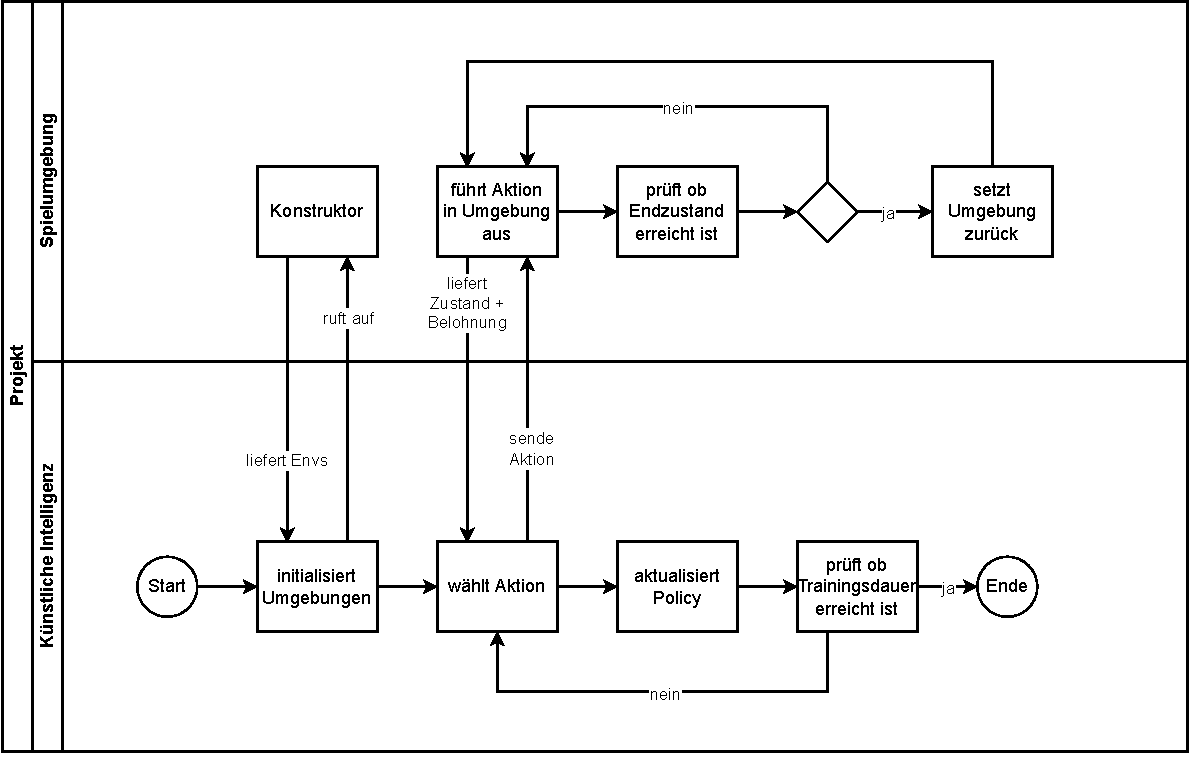
\includegraphics[width=1\textwidth]{Bilder/swimlane.drawio.pdf} 
	
	Abb. 4: Swimlane-Diagramm des Projektes \\

\end{minipage}

Der Trainingsprozess wird angestoßen, die Umgebung beziehungsweise die Umgebungen werden initialisiert. Dazu wird der Konstruktor der Umgebung aufgerufen. Daraufhin wird von der KI eine Aktion ausgewählt und an die Umgebung weitergeleitet. Die Umgebung führt diese Aktion aus und prüft ob der Endzustand des Spiels erreicht worden ist oder nicht. Wenn der Endzustand erreicht wurde wird die Umgebung auf den Anfangszustand zurückgesetzt. Wenn der Endzustand nicht erreicht worden ist, wird der Prozess ohne Weiteres fortgesetzt. Daraufhin liefert die Umgebung der KI eine Belohnung für den ausgeführten Schritt und den neuen Zustand der Umgebung nach Ausführung der Schrittes/der Aktion.

Daraufhin aktualisiert die Künstliche Intelligenz ihr neuronales Netz mit der Policy und überprüft ob bereits genügend Zeit vergangen ist, um das Training zu beenden. Wenn die festgelegte Zeit vergangen ist wird das Training an dieser Stelle beendet. Wenn nicht wird die nächste Aktion gewählt und das Training wird fortgesetzt.

Dies ist lediglich eine vereinfachte Darstellung des Prozesses. In Wirklichkeit wird die Policy nicht nach jedem Schritt/jeder Aktion aktualisiert, sondern es wird erst eine festgelegte Menge an Aktions-Zustands-Paaren gesammelt. Dann wird das neuronale Netz mit dieser Gesamtmenge aktualisiert.
\subsubsection{Die Spielumgebung}
\begin{minipage}{\linewidth}
	Die folgenden beiden Abbildungen zeigen prinzipiellen Funktionsablauf in der Spielumgebung. Dabei wird am Anfang eine Aktion entgegengenommen und am Schluss der neue Zustand dieser Umgebung nach Ausführung der Aktion zurückgegeben:\\
	
	\vspace{0.5cm}
	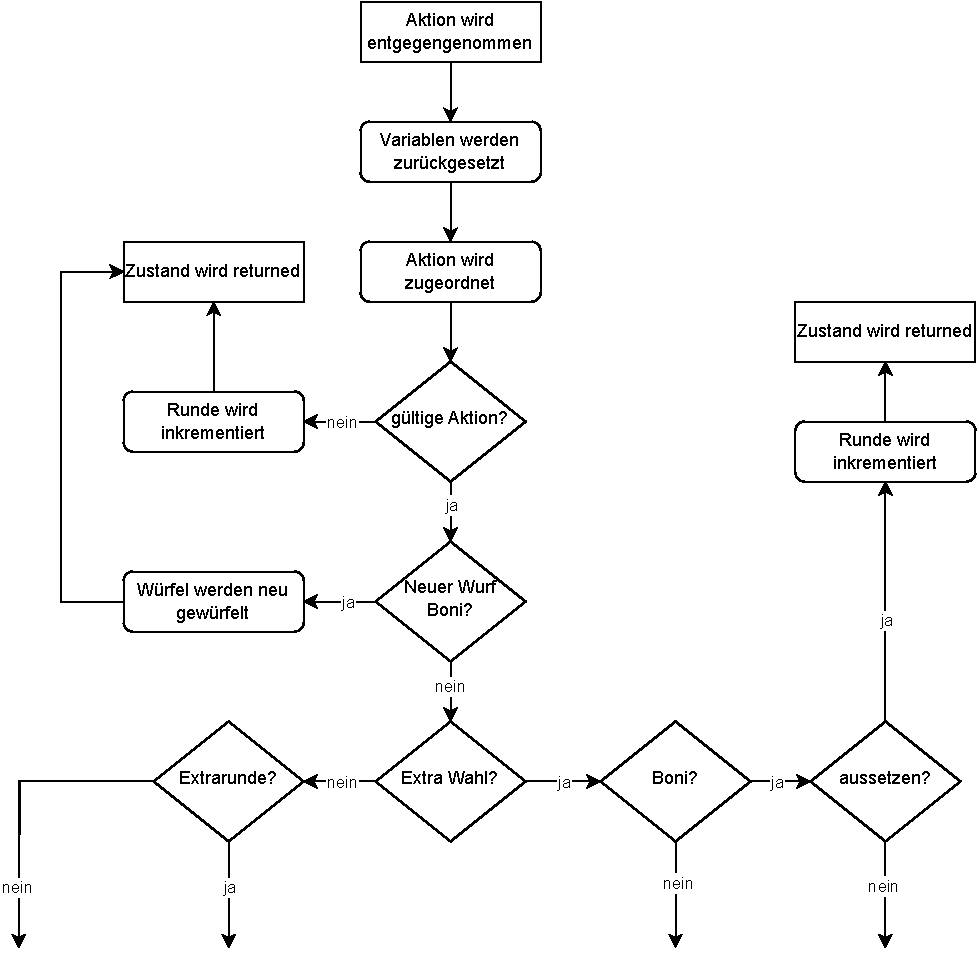
\includegraphics[width=1\textwidth]{Bilder/step3.drawio} 
	
	Abb. 5: Ablauf-Diagramm der Schritt Funktion 1 \\
\end{minipage}

Nachdem die Schritt Funktion angestoßen wird, werden die Variablen dieser Funktion zurückgesetzt, um einen klaren Schnitt zwischen vergangenen Aktionen und der aktuellen Aktion zu erzielen.

Anschließend wird die Aktion ihrem entsprechenden Ablauf zugeordnet. Es gibt Aktionen für Wahlen nach normalen Würfen, für Wahlen von Würfeln des Silbertablettes, sowie für das Nutzen von Boni. Außerdem gibt es eine Aktion, die nur dann wählbar ist, wenn keine der anderen Aktionen gewählt werden kann. Dies ist die Aktion für ungültige Züge.

Ist die Aktion nicht gültig, wird die Runde inkrementiert und der Zustand der Umgebung zurückgegeben.

Wird die Neu Würfeln Boni verwendet, werden die gültigen Würfel neu gewürfelt und anschließend der Zustand zurückgegeben.

Ist beides nicht der Fall kommt es zu einer Auswahl zwischen den wesentlichen Aktionen der Umgebung. Es gibt sogenannte Extra Wahlen, diese spalten sich auf in Extra Wahlen mit der Extra Wahl Boni und Wahlen vom Silbertablett des Mitspielers.

Handelt es sich nicht um eine Extra Wahl, so folgt eine Unterteilung in Extra Runden und Normale Runden. Bei Extra Runden wird eine der Boni verwendet, die es erlauben eines der farbigen Felder auszufüllen [siehe Grundlagen].

Handelt es sich nicht um eine Extrarunde muss es eine normale Wahl nach einem Standardwurf in einer der sechs Runden sein [siehe Grundlagen].

Handelt es sich um eine Extra Wahl mit Boni, dann steht noch die Aktion "aussetzen" zur Wahl. Diese inkrementiert lediglich die Runde, sodass das Spiel weiter fortgesetzt werden kann. Dies spiegelt die Möglichkeit im Spiel wieder auf die Nutzung der Extra Wahl Boni zu verzichten.

Der folgende Ablauf der Funktion gestaltet sich relativ ähnlich bei allen vier Varianten. Bei allen Vieren wird das Feld und das Kästchen ermittel, welches ausgefüllt werden soll und das entsprechende Kästchen wird anschließend ausgefüllt. Dann wird die Belohnung für diesen Schritt ermittelt.

Am Ende der Funktion unterscheiden sich die vier Varianten allerdings wieder. Bei der normalen Wahl nach einem Standardwurf werden die entsprechenden Würfel als ungültig markiert [siehe Grundlagen] und die Runde wird inkrementiert. Außerdem prüft die Funktion bei dieser Variante am Schluss ob das Spiel terminiert ist oder nicht.

Beim ausfüllen eines Feldes mittels Boni (keine Extra Wahl) wird der entsprechende Boni dekrementiert.

Bei der Extra Wahl vom Silbertablett wird die Runde inkrementiert.

Bei der Extra Wahl mittels Boni wird der gewählte Würfel als ungültig markiert und der Extra Wahl Boni wird dekrementiert.

Bei allen vier Varianten wird am Ende der Funktion der aktuelle Zustand der Umgebung sowie die erhaltene Belohnung für den Schritt/die Aktion zurückgegeben.\\

\begin{minipage}{\linewidth}

	\vspace{0.5cm}
	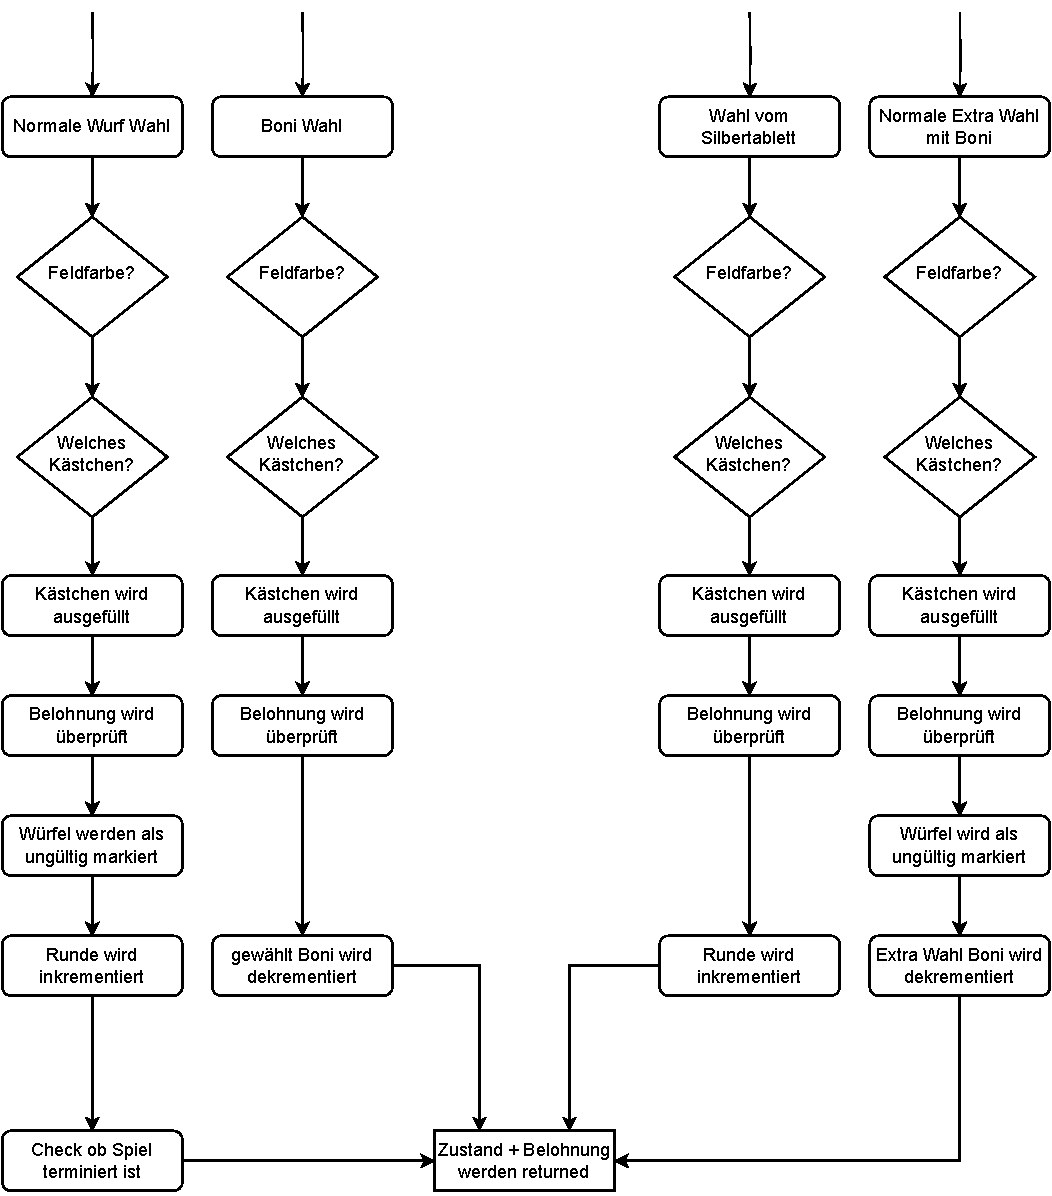
\includegraphics[width=1\textwidth]{Bilder/step2.drawio}
	
	Abb. 6: Ablauf-Diagramm der Schritt Funktion 2 \\
\end{minipage}
\subsubsection{Die Künstliche Intelligenz}
\subsubsection{Einschränkungen}
\section{Implementierung}
\subsection{Spielumgebung}
\subsubsection{Klassenattribute}
\subsubsection{Methoden}
\subsubsection{Einzelne Methoden...}
\subsection{AI}
\subsubsection{Model Learn}
\subsubsection{Model Predict}
\subsubsection{Init Envs}
\subsection{Darstellung}
\subsubsection{Make Entry}
\subsubsection{Plot History}
\subsection{Verwendung}
\section{Ergebnisse}
In diesem Kapitel werden die Ergebnisse des Projektes vorgestellt. Dabei werden sowohl der Verlauf der Implementierungsphase als auch die Finalen Ergebnisse dieser behandelt. Zunächst wurde ein Prototyp entwickelt, der die wesentlichen Funktionalitäten des Modells und der Spielumgebung beinhaltet, um sicherzustellen dass das vorhaben im Rahmen der Vorgaben umsetzbar ist und um Einblicke in mögliche Problemstellungen, welche sich mit der Umsetzung des Projektes ergeben könnten, zu erhalten. Danach wurde der Prototyp Stück für Stück erweitert, bis schließlich das komplette Spiel mit all seinen Funktionalitäten umgesetzt worden ist und das Modell damit trainiert werden konnte.
\subsection{Trainingshistorie}
\subsubsection{Version 1.1.0}
Bei dieser Version handelt es sich um den ersten lauffähigen Prototypen der Umgebung. Es ist nur eines der farbigen Felder (das gelbe) in der Spielumgebung implementiert worden. Das Modell kann mithilfe dieser Spielumgebung bereits trainiert werden und erzielt 
\subsubsection{Version 2.0}
\subsubsection{Version 3.0}
\subsubsection{Version 4.0}
\subsection{Finale Ergebnisse}
\subsubsection{Performance}
\subsubsection{Hyperparameter}
\subsubsection{ChatGPT 4}
\section{Zusammenfassung und Ausblick}

Insgesamt lässt sich sagen, dass das Projekt ein Erfolg war. Es ließ sich eine Künstliche Intelligenz mithilfe relativ einfacher Methoden für das Spiel Ganz schön clever implementieren und diese erzielte sehr gute Ergebnisse. 

Besonders hilfreich war es einen Prototypen zu bauen und von diesem Punkt an weiterzuarbeiten. Dies half dabei leichter einen Überblick über die wichtigsten Aspekte zu gewinnen und diese auch umzusetzen, statt ausschweifend zu planen. 

Die Implementierung der Künstlichen Intelligenz selbst gestaltete sich dank Bibliotheken wie Gymnasium und Stable Baselines vergleichsweise einfach, brachte aber dennoch eine Vielzahl interessanter und nützlicher Erkenntnisse mit sich. Besonders hervorzuheben ist dabei die Anpassung von Hyperparametern, welche zum Teil zu sehr unterschiedlichen Ergebnissen geführt hat. 

Der Aufwändigste Teil des Projektes war die Implementierung des Spielumgebung selbst. Das Spiel hat viele kleine Interaktionen, welche zum Teil ineinander verschachtelt sind und es gestaltete sich zum Teil schwierig alle Zusammenhänge zu überschauen und zu gewährleisten, dass Änderungen an einer Funktion andere nicht negativ beeinflusst. Es sind auch vielerlei Bugs aufgetreten, welche gefunden und behoben werden mussten. Der gravierendste Fehler war es das Runden-System nicht von vornherein zu implementieren, sondern es später einzufügen, als die meisten anderen Aspekte des Spiels bereits implementiert waren. Dies führte dazu, dass viele Aspekte der Spielumgebung neu überdacht und überarbeitet werden mussten. Für die Zukunft bleibt zu sagen, dass man sich auf alle grundlegenden Aspekte des Spiels/Problems konzentrieren und diese lauffähig machen sollte, bevor man anfängt bereits Funktionierende Aspekte zu erweitern. Der Einfluss einer Änderung des Runden-Systems wurde unterschätzt.\\

Für die Weiterarbeit am Projekt schlage ich vor, eine grafische Visualisierung des Lern- oder Vorhersageprozesses zu implementieren. Außerdem lässt sich das Modell sicherlich mithilfe anderen Algorithmen, Trainingsverfahren oder Hyperparameter weiter optimieren. Was im Rahmen der Arbeit ebenfalls nur bedingt erfolgt ist, ist eine Analyse der Spielstrategien von Modellen und wie sich unterschiedliche Strategien auf die Performance auswirken. Zwar wurden Variablen hinzugefügt, welche messen, wie oft Kästchen in bestimmten Feldern ausgefüllt wurden, allerdings lässt sich hier noch viel mehr machen. Ebenfalls wäre es sinnvoll Tests für das Projekt zu implementieren, um sicherzustellen, dass alle Aspekte der Umgebung wie vorhergesehen funktionieren und zusammenarbeiten. Zwar erfolgten Tests durch die Auswertung von Umgebungsvariablen und Print-Statements, aber fehlt dem Projekt eine fundierte Umsetzung professioneller Testverfahren.

\finishHSCdocument